\documentclass[10pt,aspectratio=169]{beamer}
\usepackage[utf8]{inputenc}
\usepackage[spanish]{babel}
\usepackage{graphicx}
\usepackage{booktabs}
\usepackage{amsmath}
\usepackage{multirow}
\usepackage{xcolor}

\usetheme{Madrid}
\usecolortheme{default}

\setbeamertemplate{caption}[numbered]
\setbeamertemplate{navigation symbols}{}

\title[Heart Disease -- Análisis de Datos]
      {Análisis Exploratorio y Minería de Datos\\
       sobre Heart Disease Dataset (UCI)}
\subtitle{Proyecto ADD -- 2026}
\author{Felipe}
\institute{Universidad -- Análisis de Datos}
\date{\today}

\begin{document}

% ============================================================
% PORTADA
% ============================================================
\begin{frame}[plain]
  \titlepage
\end{frame}

% ============================================================
% ÍNDICE
% ============================================================
\begin{frame}{Contenido}
  \tableofcontents
\end{frame}

% ============================================================
% SECCIÓN 1: LIMPIEZA Y PREPROCESAMIENTO
% ============================================================
\section{Limpieza y preprocesamiento}

\begin{frame}{Exploración inicial (EDA)}
  \begin{itemize}
    \item \textbf{Dataset:} Heart Disease (UCI, id=45), 303 registros, 14 variables.
    \item \textbf{Target:} Severidad de enfermedad cardíaca (0--4).
    \item \textbf{Variables clave:} age, chol, trestbps, thalach, oldpeak.
  \end{itemize}

  \begin{center}
    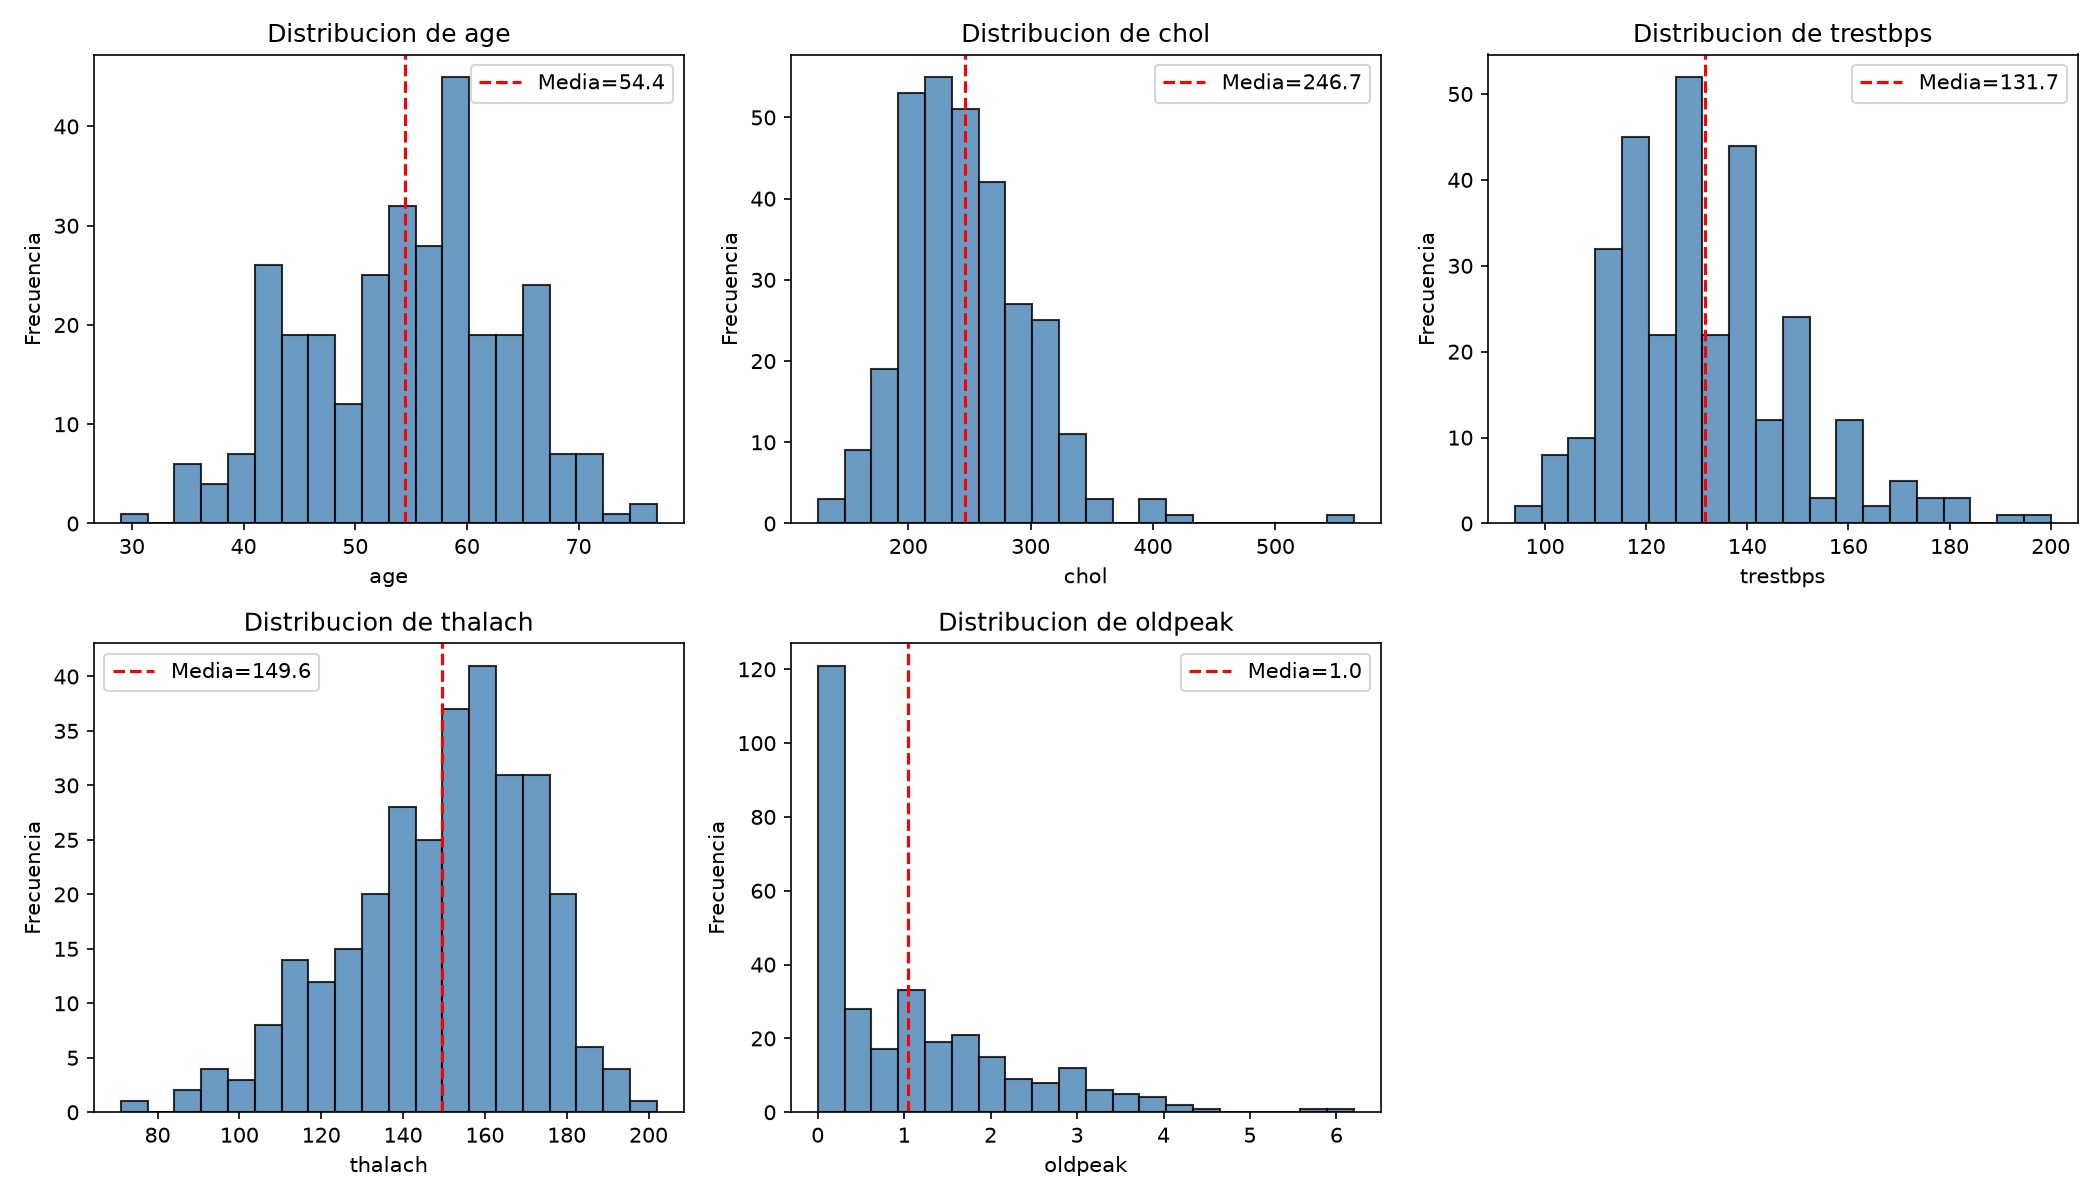
\includegraphics[height=0.45\textheight]{../plots/1_seleccion_eda/histogramas.png}
  \end{center}

  \textbf{Observación:} Distribuciones asimétricas en chol y oldpeak; presencia de outliers visibles.
\end{frame}

\begin{frame}{Boxplots y detección de outliers}
  \begin{columns}
    \column{0.50\textwidth}
      \centering
      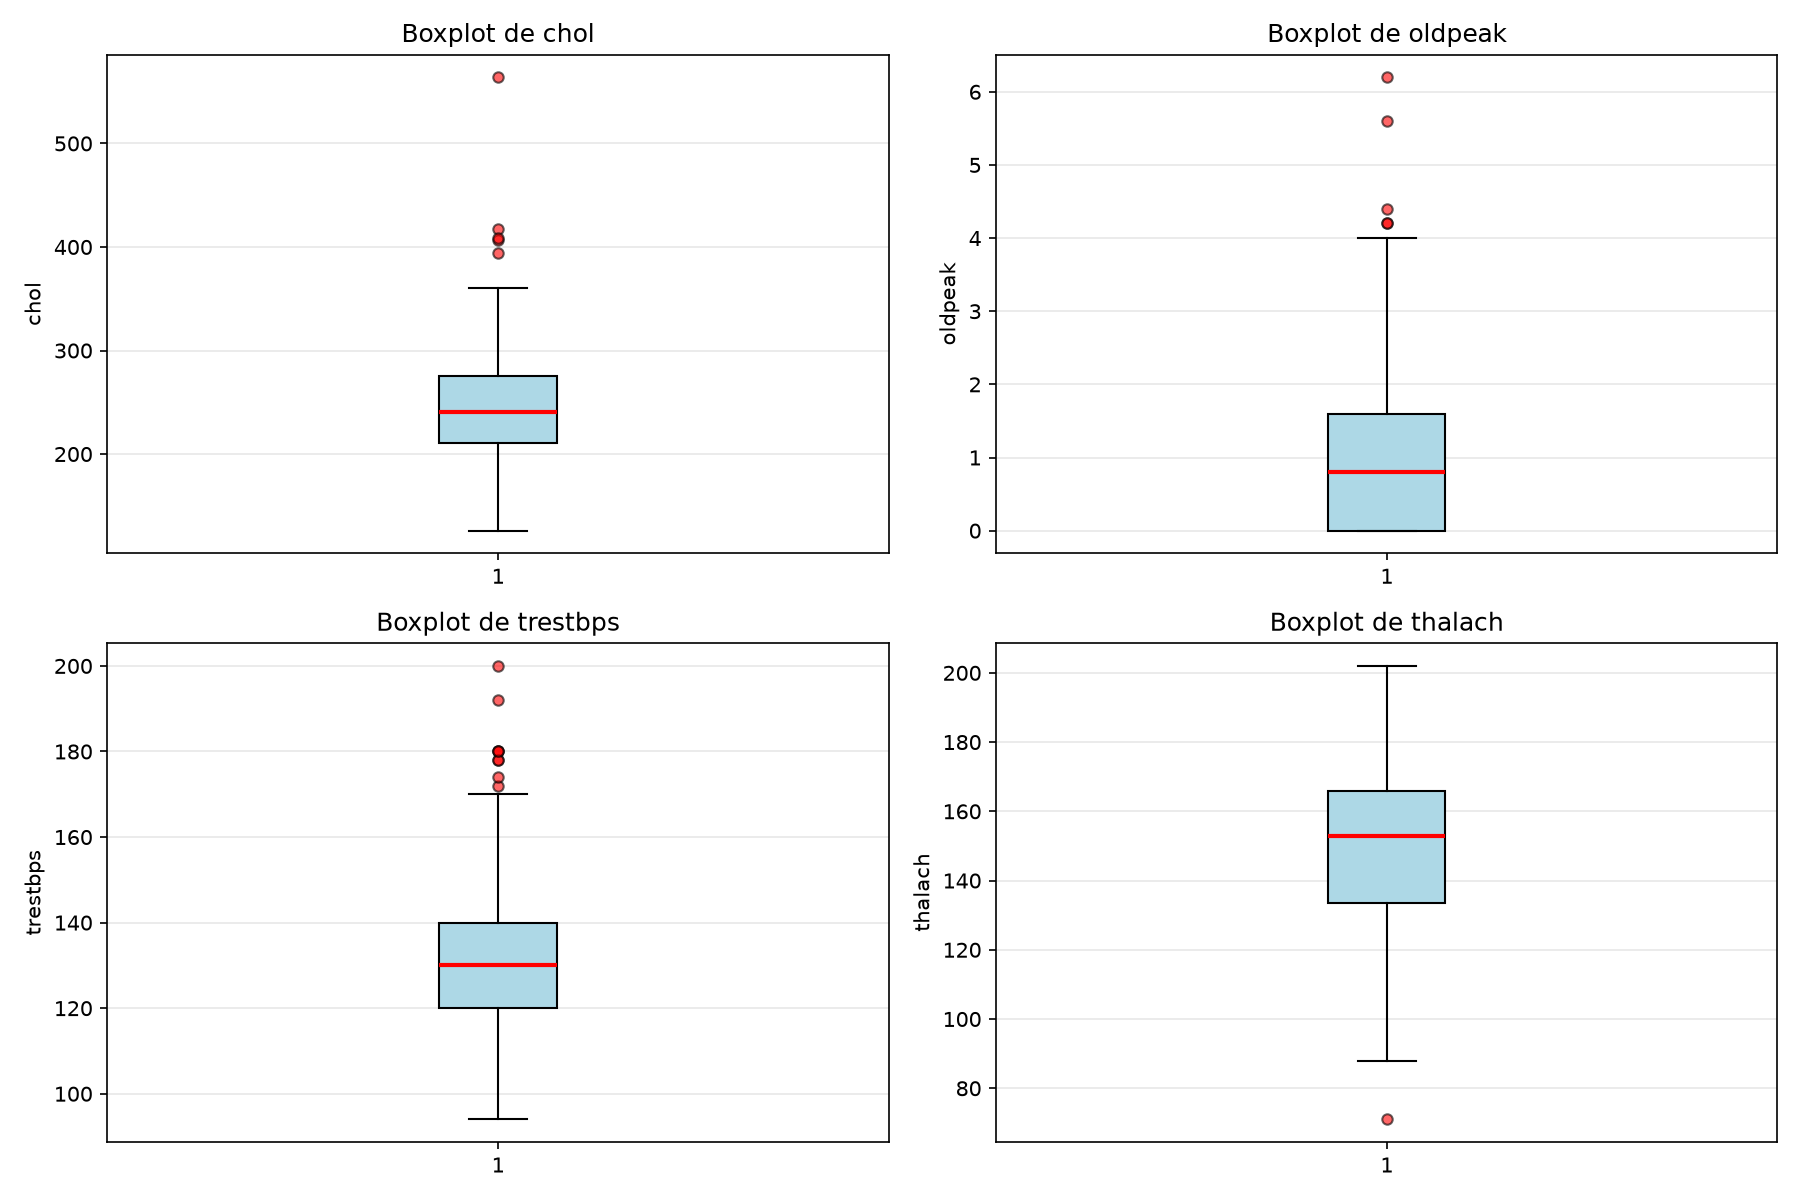
\includegraphics[width=\textwidth]{../plots/1_seleccion_eda/boxplots.png}
      \textbf{Boxplots individuales}

    \column{0.50\textwidth}
      \centering
      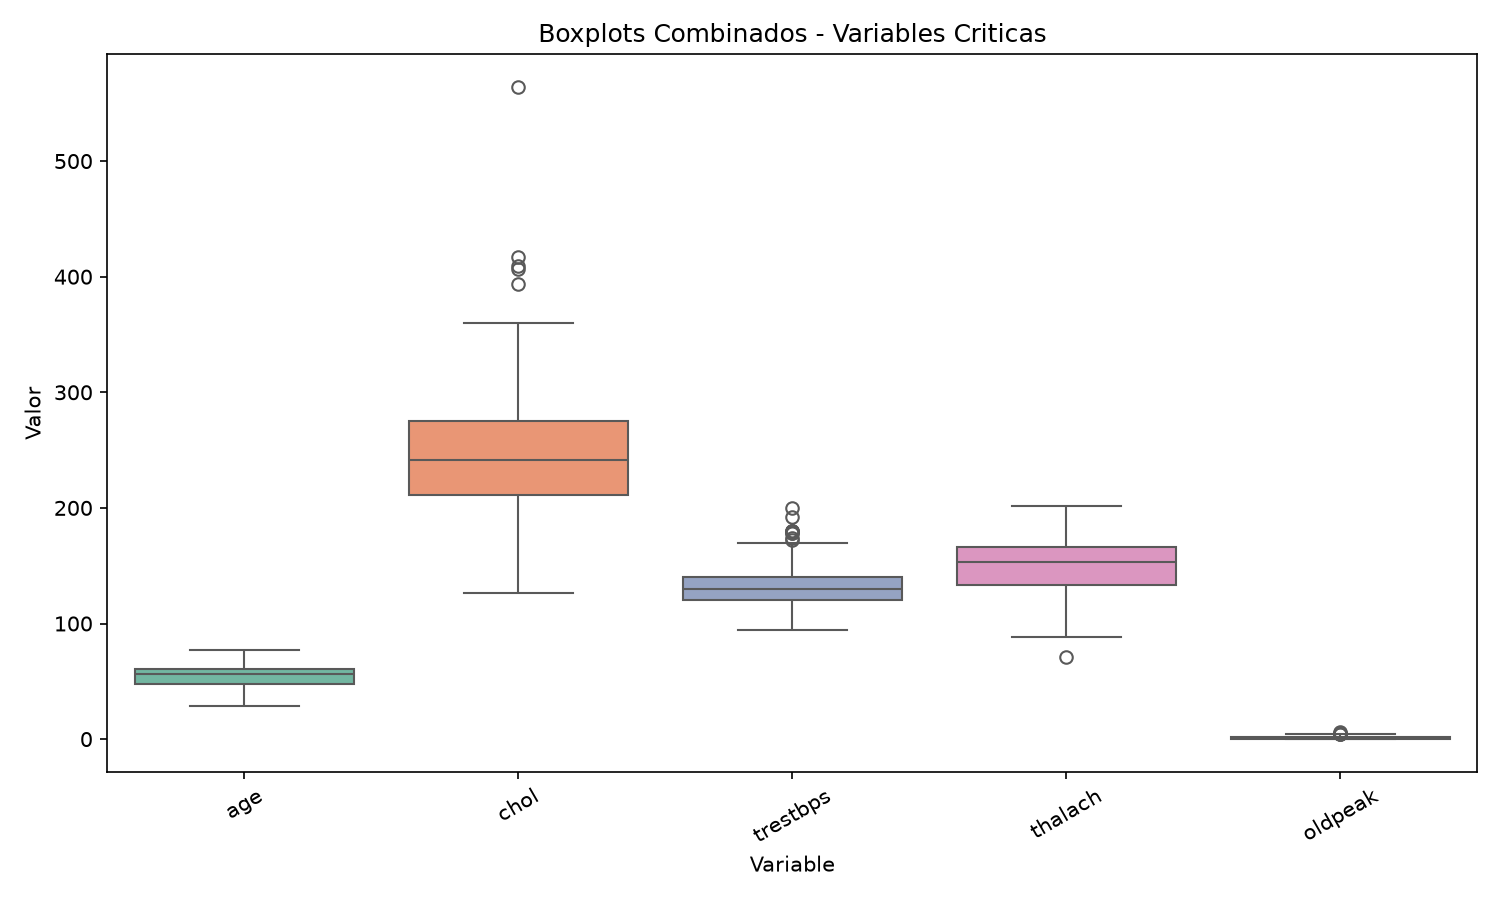
\includegraphics[width=\textwidth]{../plots/1_seleccion_eda/boxplots_combinados.png}
      \textbf{Boxplots combinados}
  \end{columns}

  \vspace{0.3cm}
  \begin{itemize}
    \item chol y oldpeak presentan la mayor cantidad de valores atípicos.
    \item trestbps y thalach muestran dispersiones controladas.
  \end{itemize}
\end{frame}

\begin{frame}{Matriz de correlación}
  \begin{center}
    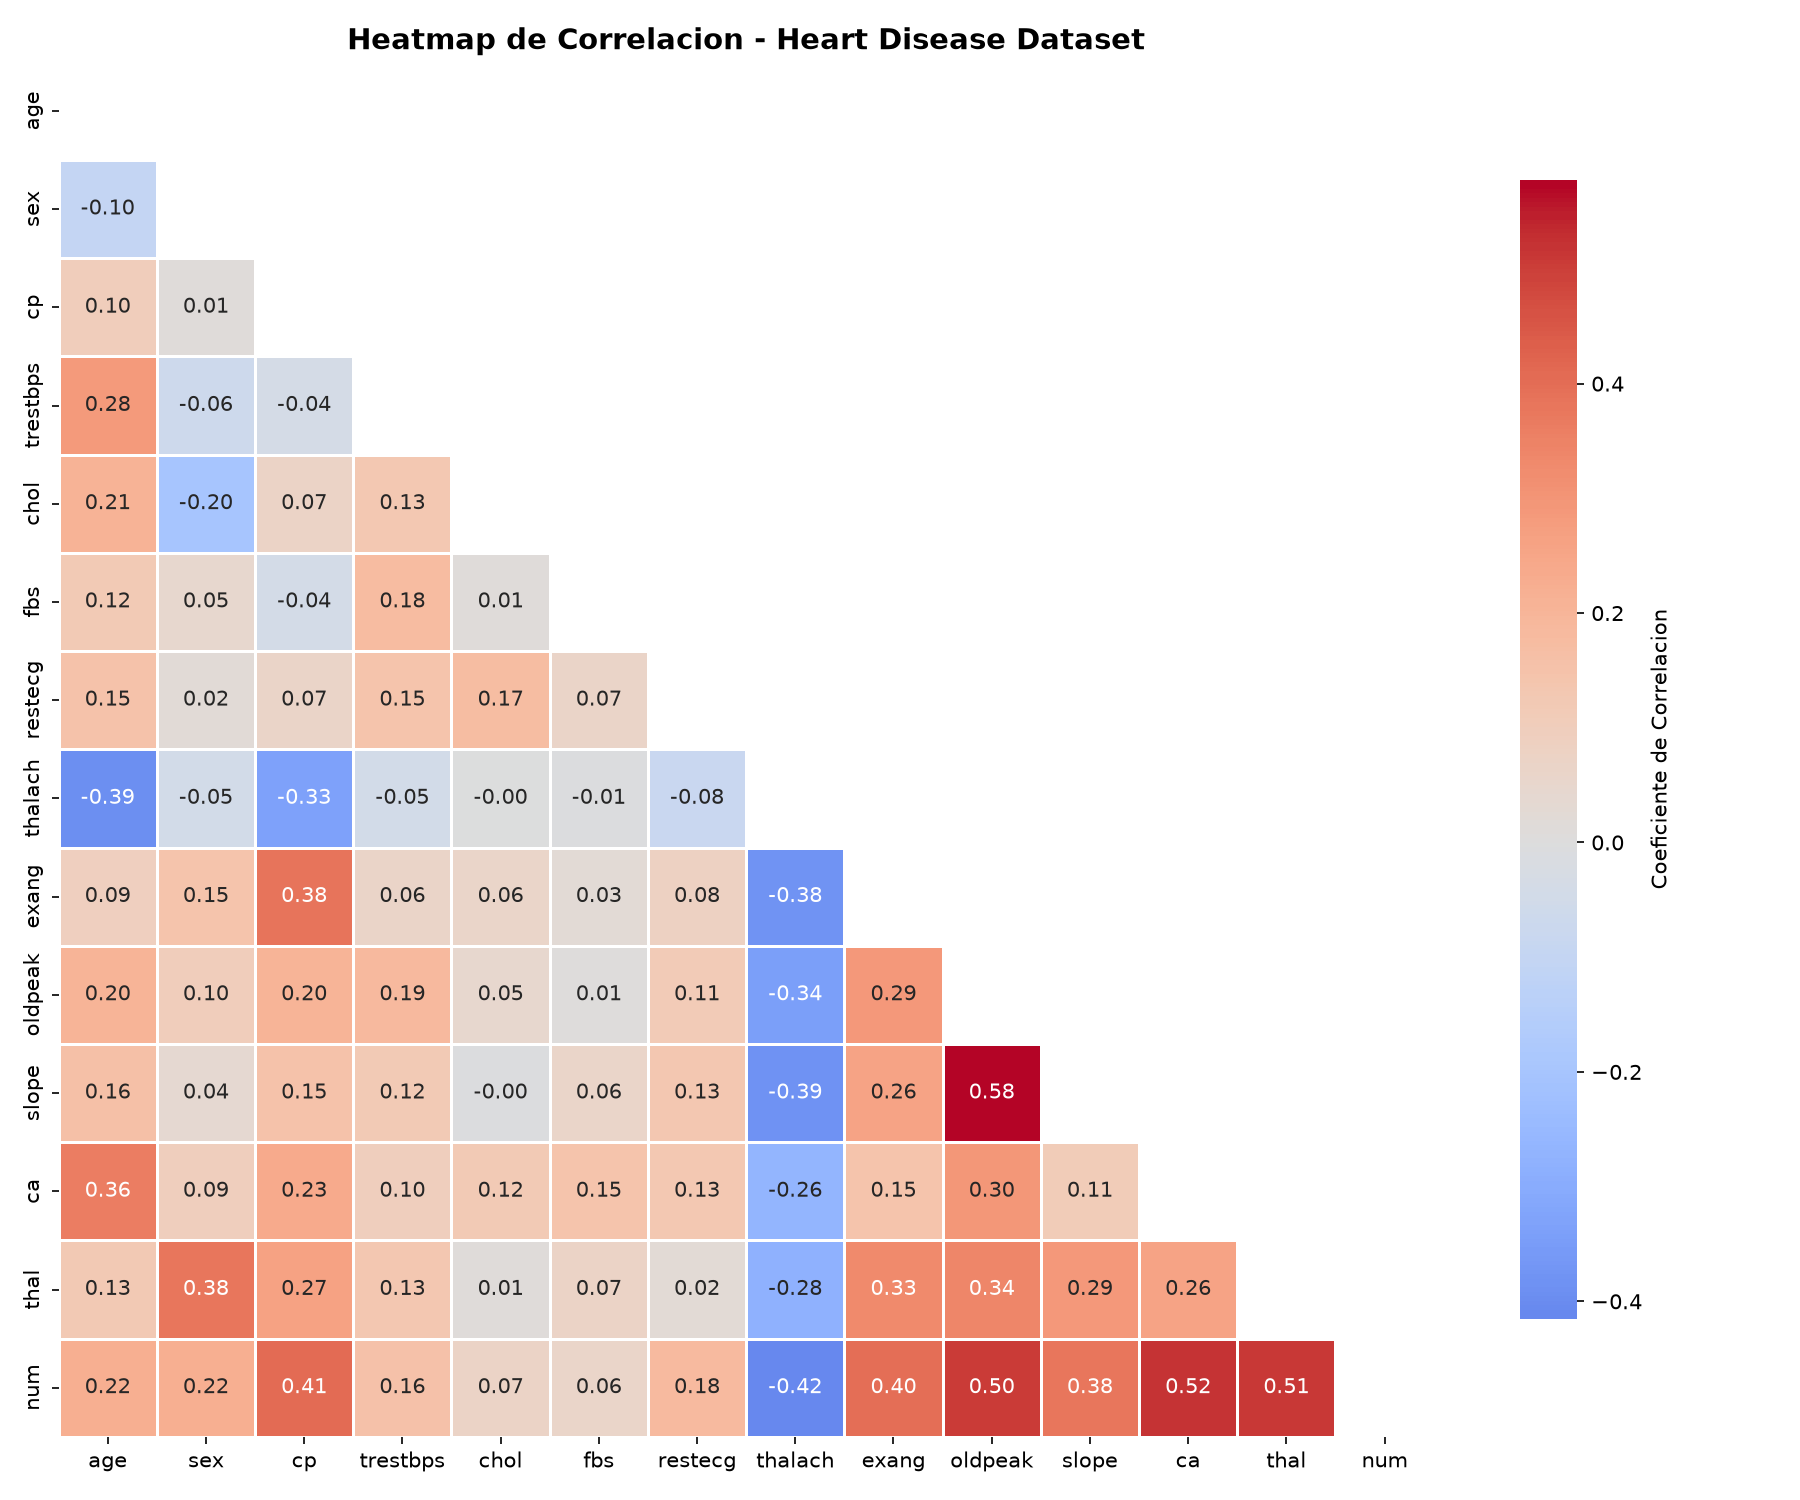
\includegraphics[height=0.65\textheight]{../plots/1_seleccion_eda/heatmap_correlacion.png}
  \end{center}

  \begin{itemize}
    \item Correlaciones moderadas: ninguna supera $|r| > 0.6$ (máx. 0.578 entre oldpeak y slope), descartando multicolinealidad severa.
    \item \texttt{ca}, \texttt{thal} y \texttt{oldpeak} son las más correlacionadas con el target.
  \end{itemize}
\end{frame}

\begin{frame}{Tratamiento de valores nulos y codificación}
  \textbf{Valores nulos detectados:}
  \begin{itemize}
    \item \texttt{ca}: 4 nulos $\rightarrow$ imputados con la mediana.
    \item \texttt{thal}: 2 nulos $\rightarrow$ imputados con la moda.
  \end{itemize}

  \vspace{0.3cm}
  \textbf{Codificación de variables categóricas:}
  \begin{itemize}
    \item \textbf{Binarias} (sex, fbs, exang): mantenidas como 0/1.
    \item \textbf{Multi-categoría} (cp, restecg, slope, thal): One-Hot Encoding.
    \item \textbf{Continuas} (age, trestbps, chol, thalach, oldpeak, ca): solo escalado.
  \end{itemize}
\end{frame}

\begin{frame}{Eliminación de outliers (IQR)}
  \begin{center}
    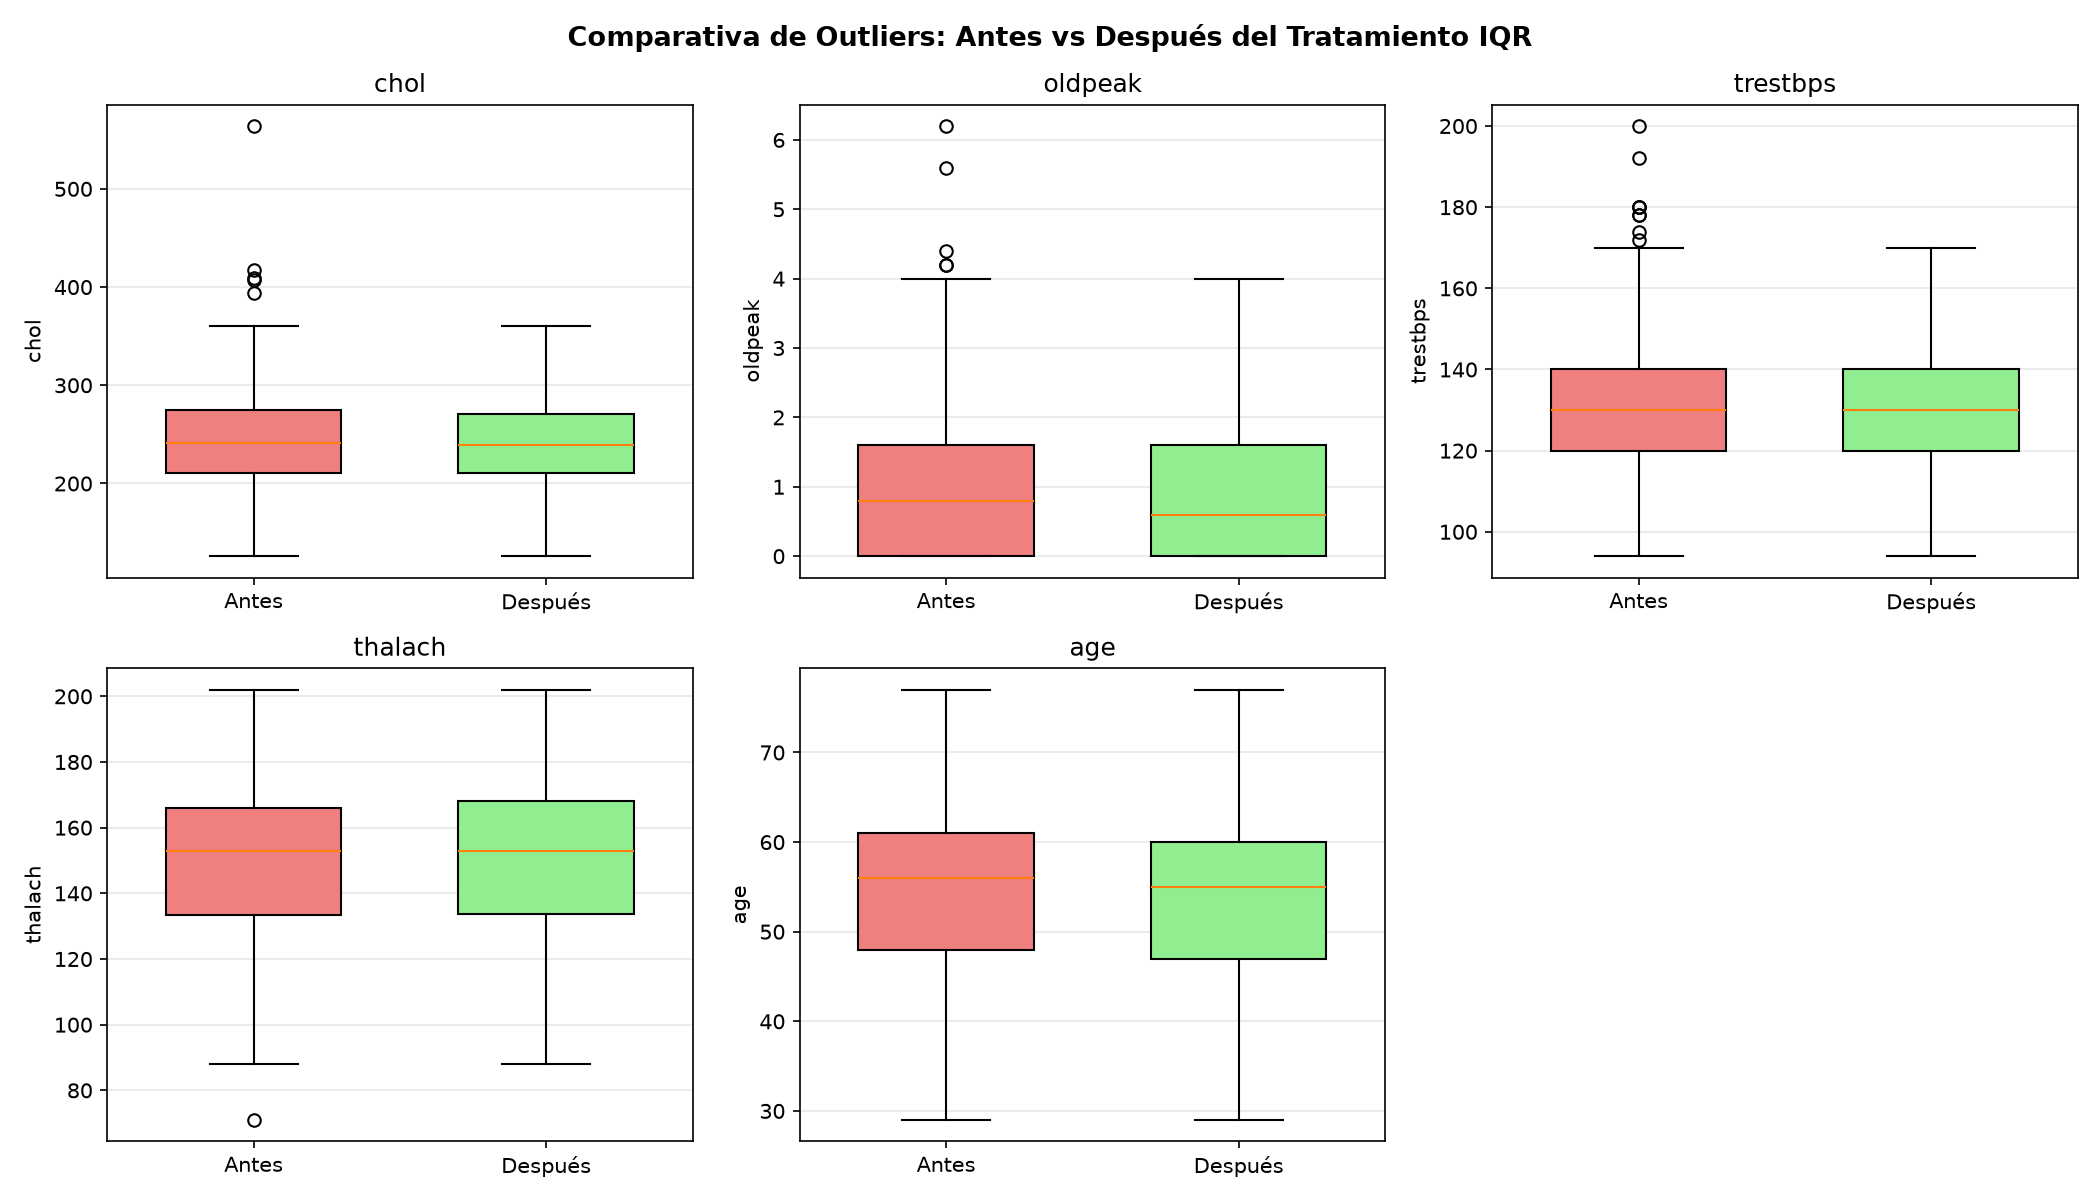
\includegraphics[height=0.55\textheight]{../plots/2_preprocesamiento/outliers_antes_despues.png}
  \end{center}

  \begin{itemize}
    \item Método IQR ($Q_1 - 1.5\cdot IQR$, $Q_3 + 1.5\cdot IQR$) aplicado sobre 5 variables continuas.
    \item \textbf{Resultado:} 19 filas eliminadas (combinadas). Shape final: 284 filas $\times$ 22 columnas (tras one-hot).
    \item Las cajas verdes (``Después'') muestran distribuciones más limpias y compactas.
  \end{itemize}
\end{frame}

\begin{frame}{Estandarización (StandardScaler)}
  \begin{itemize}
    \item Todas las variables fueron escaladas a media $\mu = 0$ y desviación $\sigma = 1$.
    \item \textbf{Justificación:} PCA y algoritmos basados en distancia (OPTICS, k-NN) requieren variables en la misma escala.
  \end{itemize}

  \vspace{0.5cm}
  \begin{block}{Resumen del preprocesamiento}
    \begin{center}
    \begin{tabular}{lcc}
      \toprule
      \textbf{Etapa} & \textbf{Antes} & \textbf{Después} \\
      \midrule
      Carga inicial      & 303 $\times$ 14 & -- \\
      Imputación de nulos & 6 nulos & 0 nulos \\
      Eliminación outliers & 303 filas & 284 filas \\
      One-Hot Encoding    & 14 columnas & 22 columnas \\
      Escalamiento        & Escalas heterogéneas & $\mu=0, \sigma=1$ \\
      \bottomrule
    \end{tabular}
    \end{center}
  \end{block}
\end{frame}

% ============================================================
% SECCIÓN 2: REDUCCIÓN DIMENSIONAL
% ============================================================
\section{Reducción dimensional}

\begin{frame}{PCA: Varianza explicada y Scree Plot}
  \begin{center}
    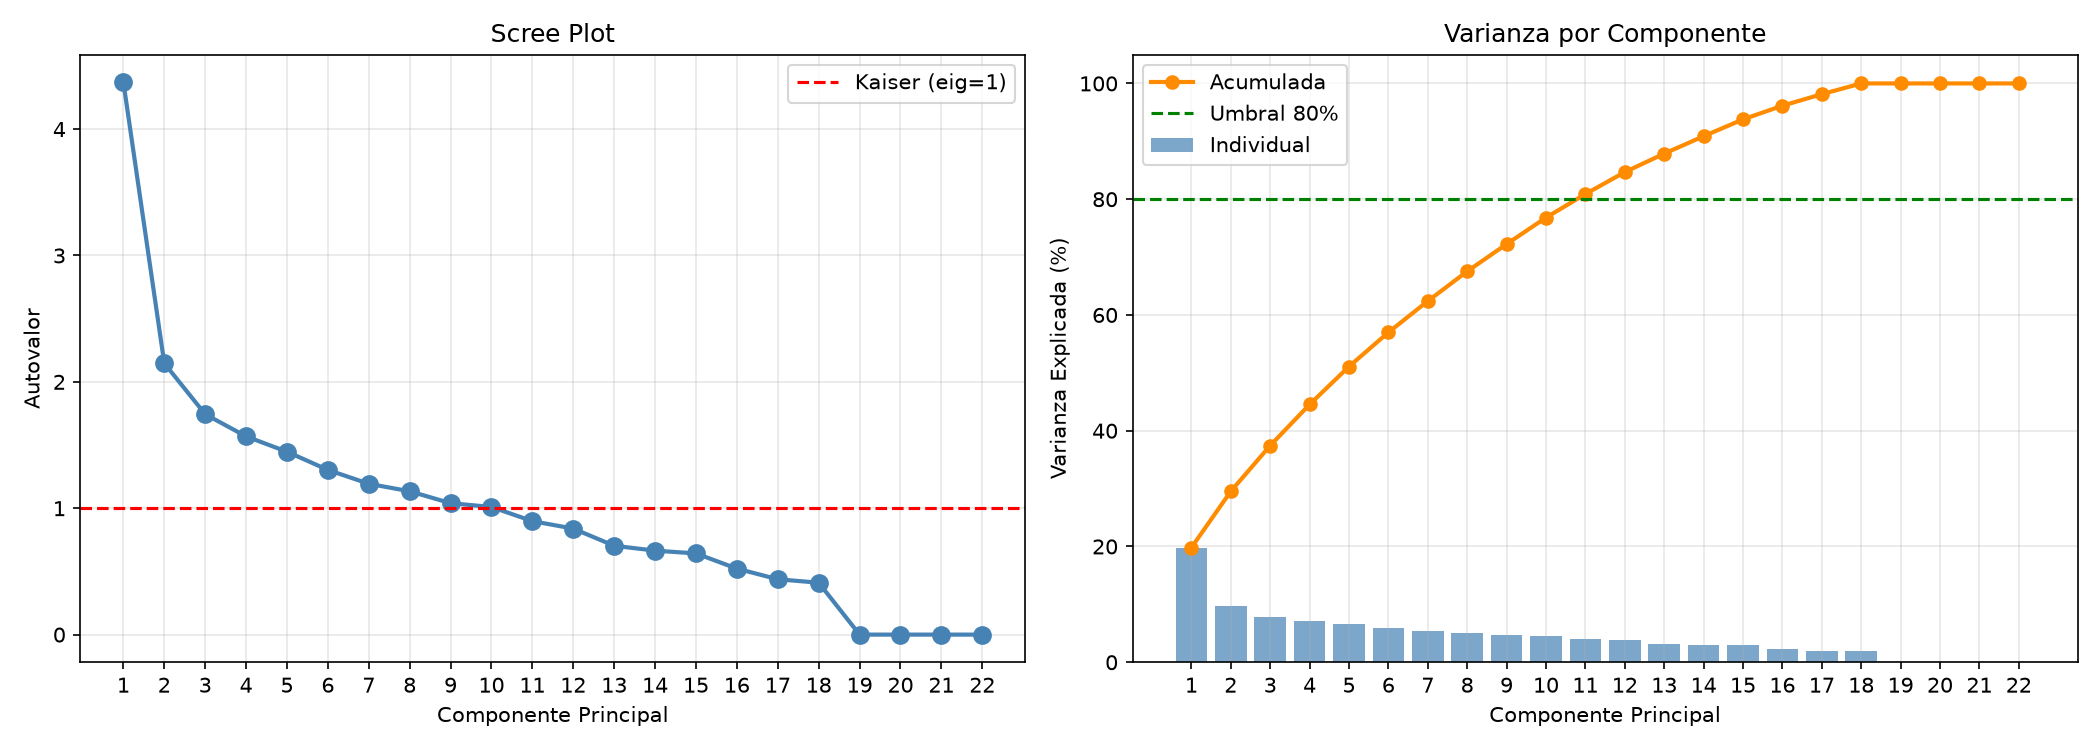
\includegraphics[height=0.65\textheight]{../plots/3_transformacion/pca_varianza.png}
  \end{center}

  \begin{itemize}
    \item \textbf{Criterio de Kaiser} (eigenvalue $>1$): 10 componentes retenidos (76.8\% de varianza acumulada).
    \item \textbf{Umbral 80\%:} Se requieren 11 de 22 componentes -- estructura mayoritariamente NO lineal.
  \end{itemize}
\end{frame}

\begin{frame}{PCA: Loadings -- contribución de variables}
  \begin{center}
    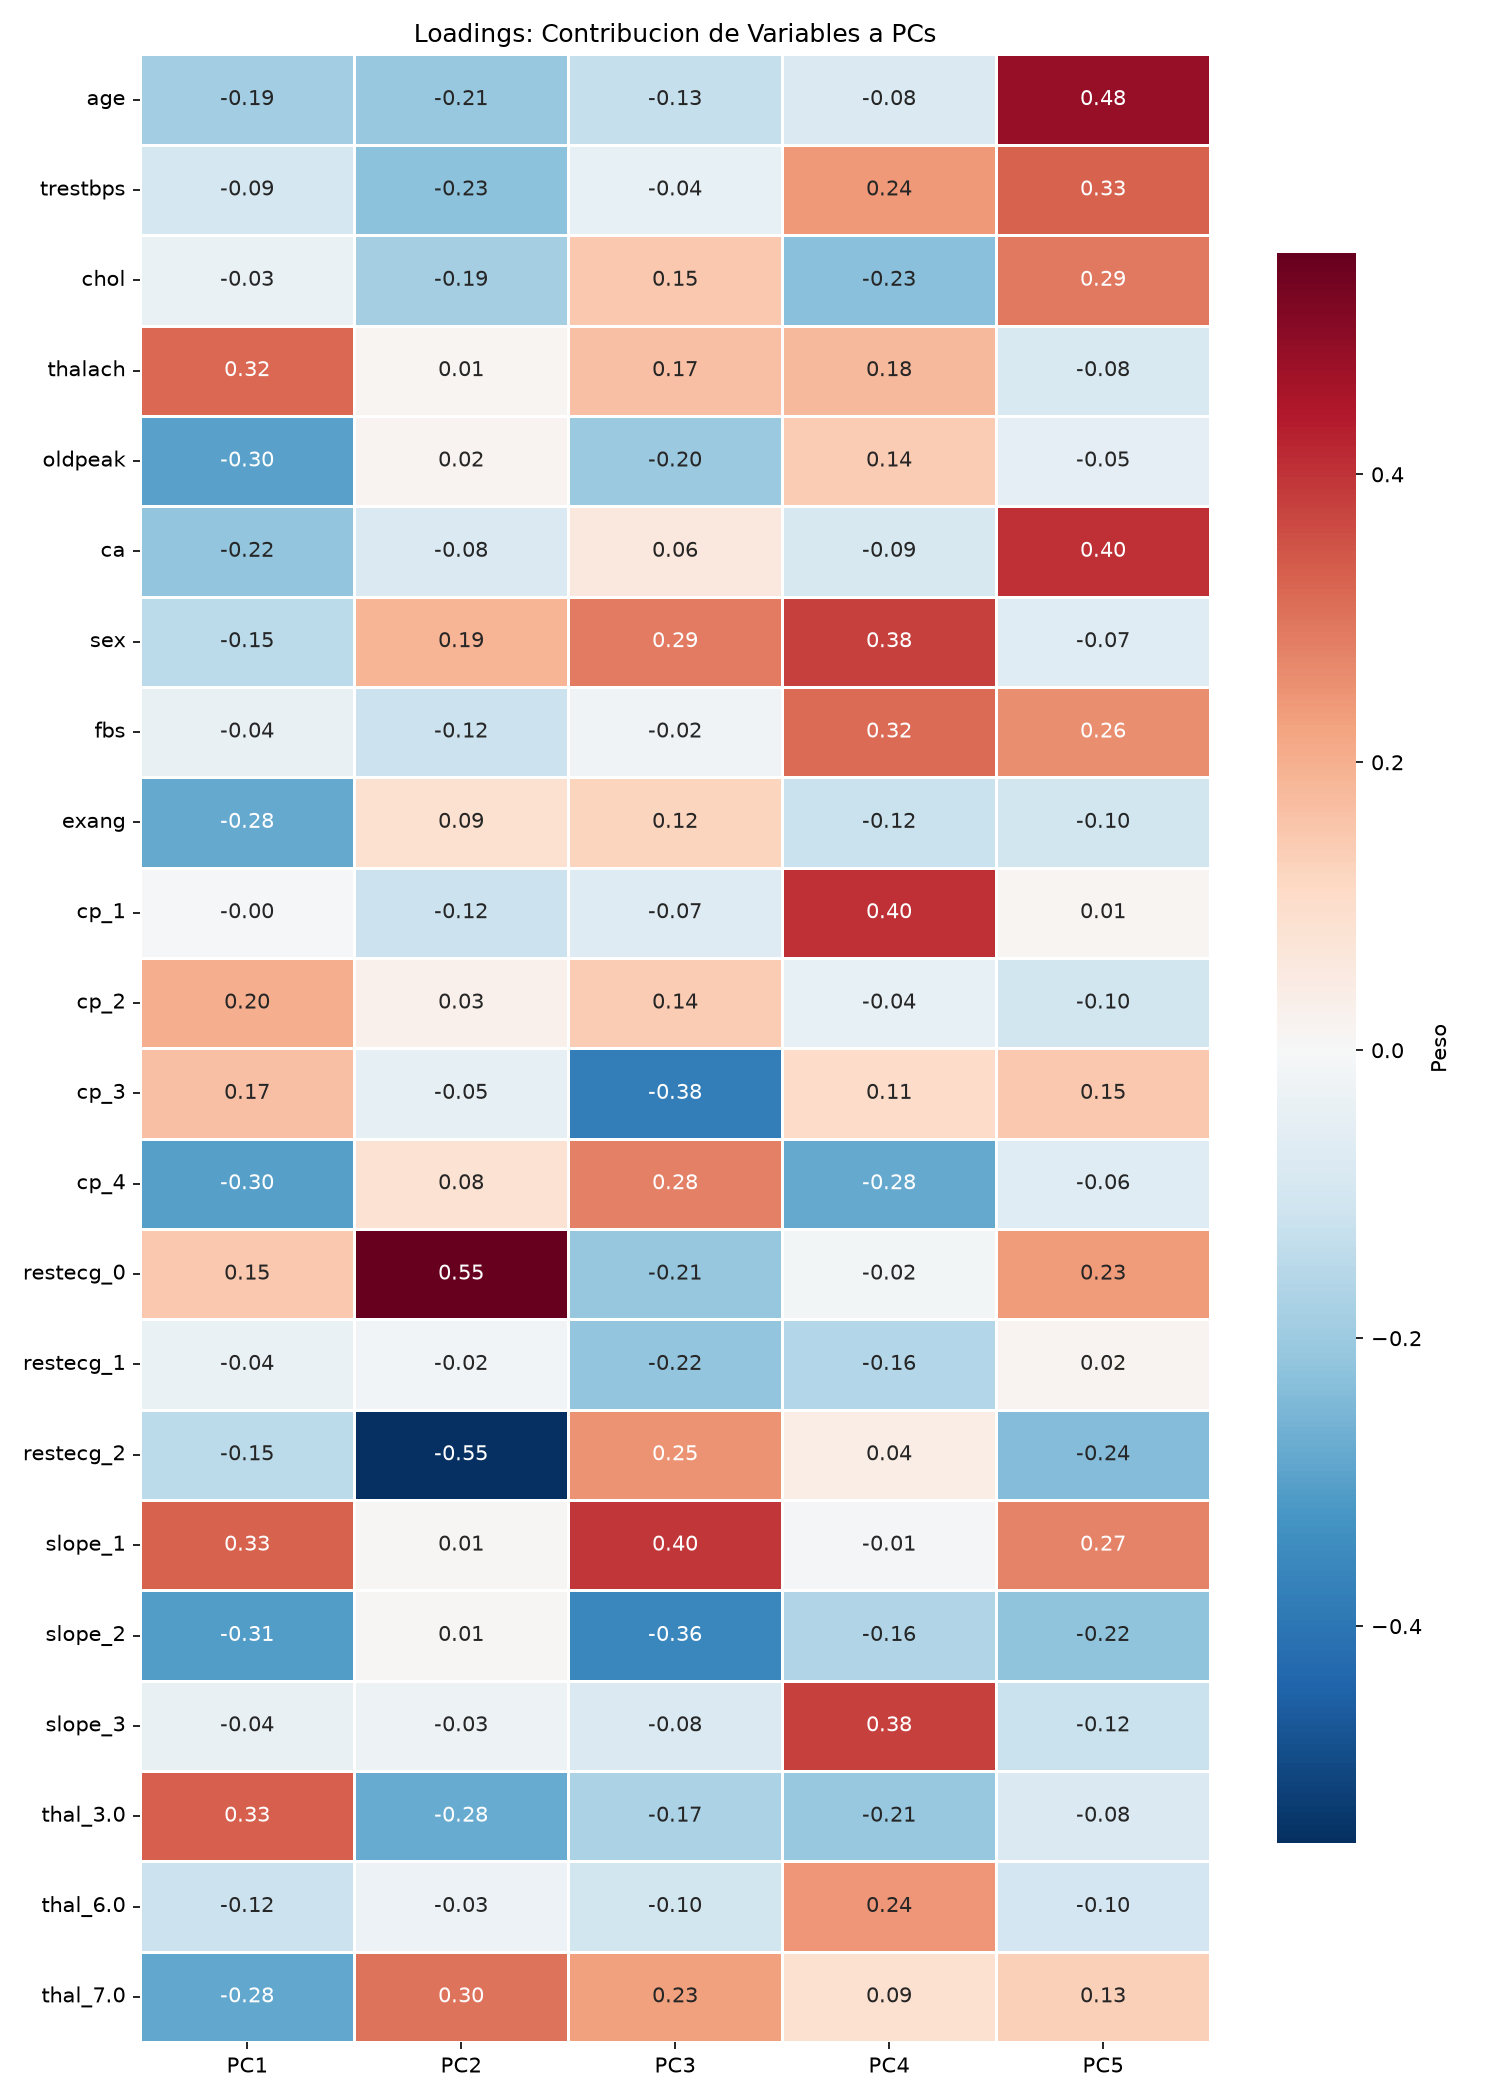
\includegraphics[height=0.65\textheight]{../plots/3_transformacion/pca_loadings.png}
  \end{center}

  \begin{itemize}
    \item \textbf{PC1:} Dominada por thalach, slope y thal (y, en sentido inverso, por oldpeak, exang y cp\_4).
    \item \textbf{PC2:} Pesos fuertes en restecg (alteraciones de reposo) y variables de thal.
    \item Las variables one-hot del cp y slope tienen contribuciones relevantes en PC3--PC5.
  \end{itemize}
\end{frame}

\begin{frame}{PCA: Proyección 2D}
  \begin{center}
    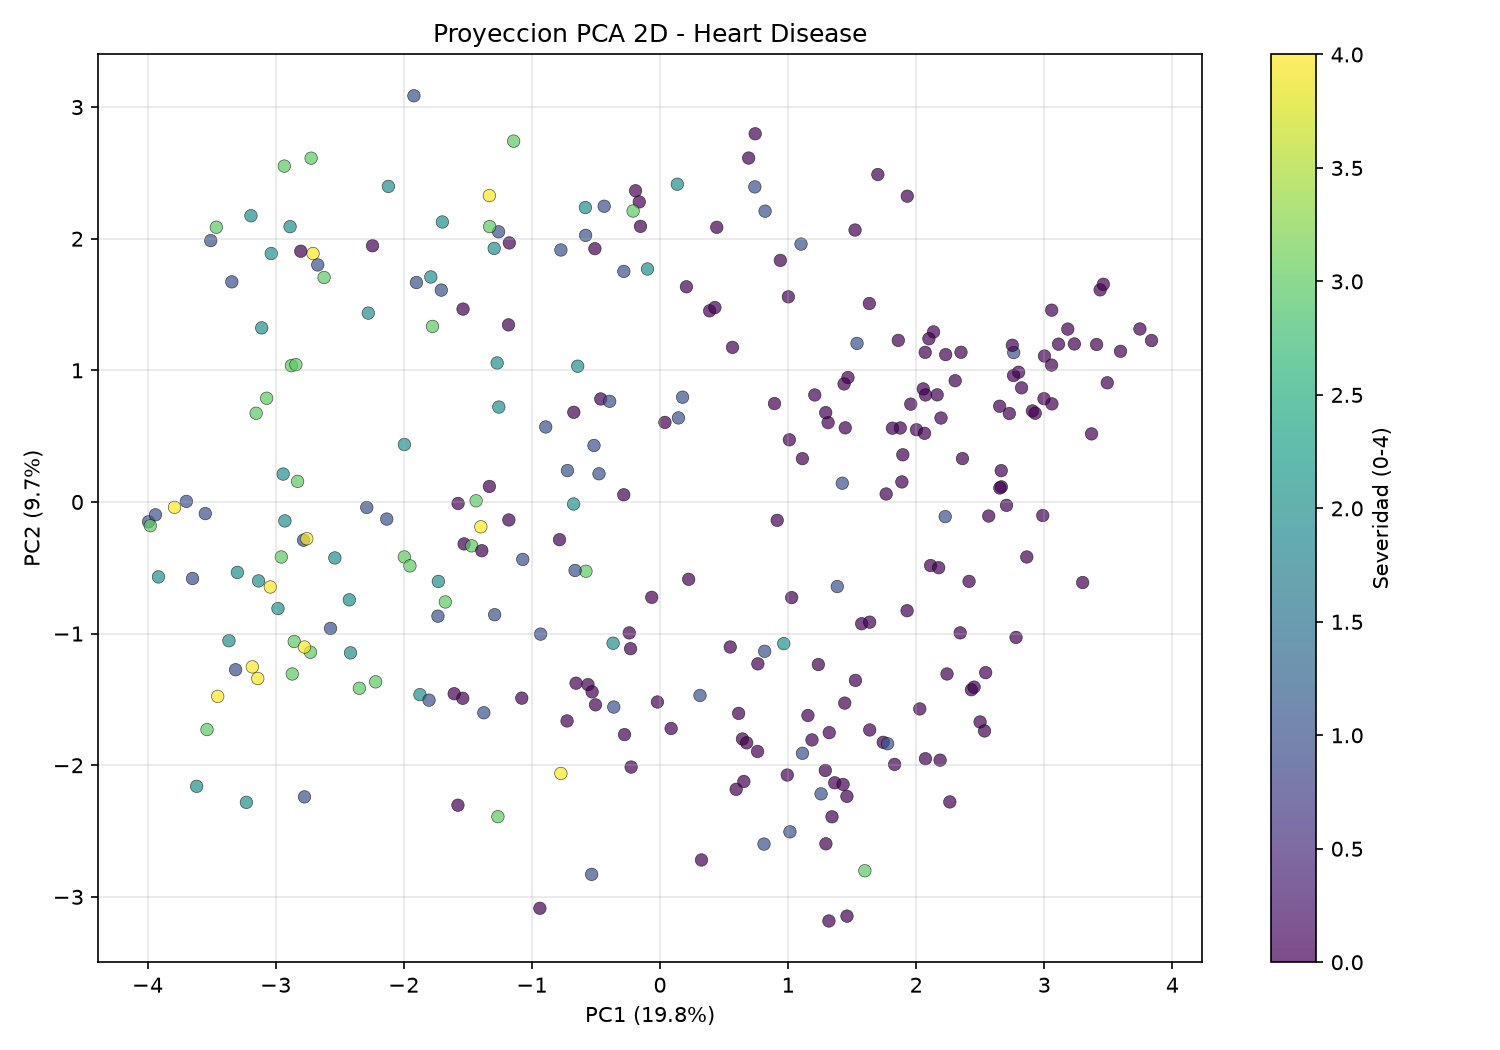
\includegraphics[height=0.60\textheight]{../plots/3_transformacion/pca_proyeccion_2d.png}
  \end{center}

  \begin{itemize}
    \item Varianza explicada en 2D: $\approx 29.5\%$ (PC1 + PC2).
    \item Las clases de severidad (0--4) no se separan linealmente en las dos primeras componentes.
    \item Justifica la exploración de métodos no lineales.
  \end{itemize}
\end{frame}

\begin{frame}{UMAP: Hiperparámetros}
  \begin{center}
    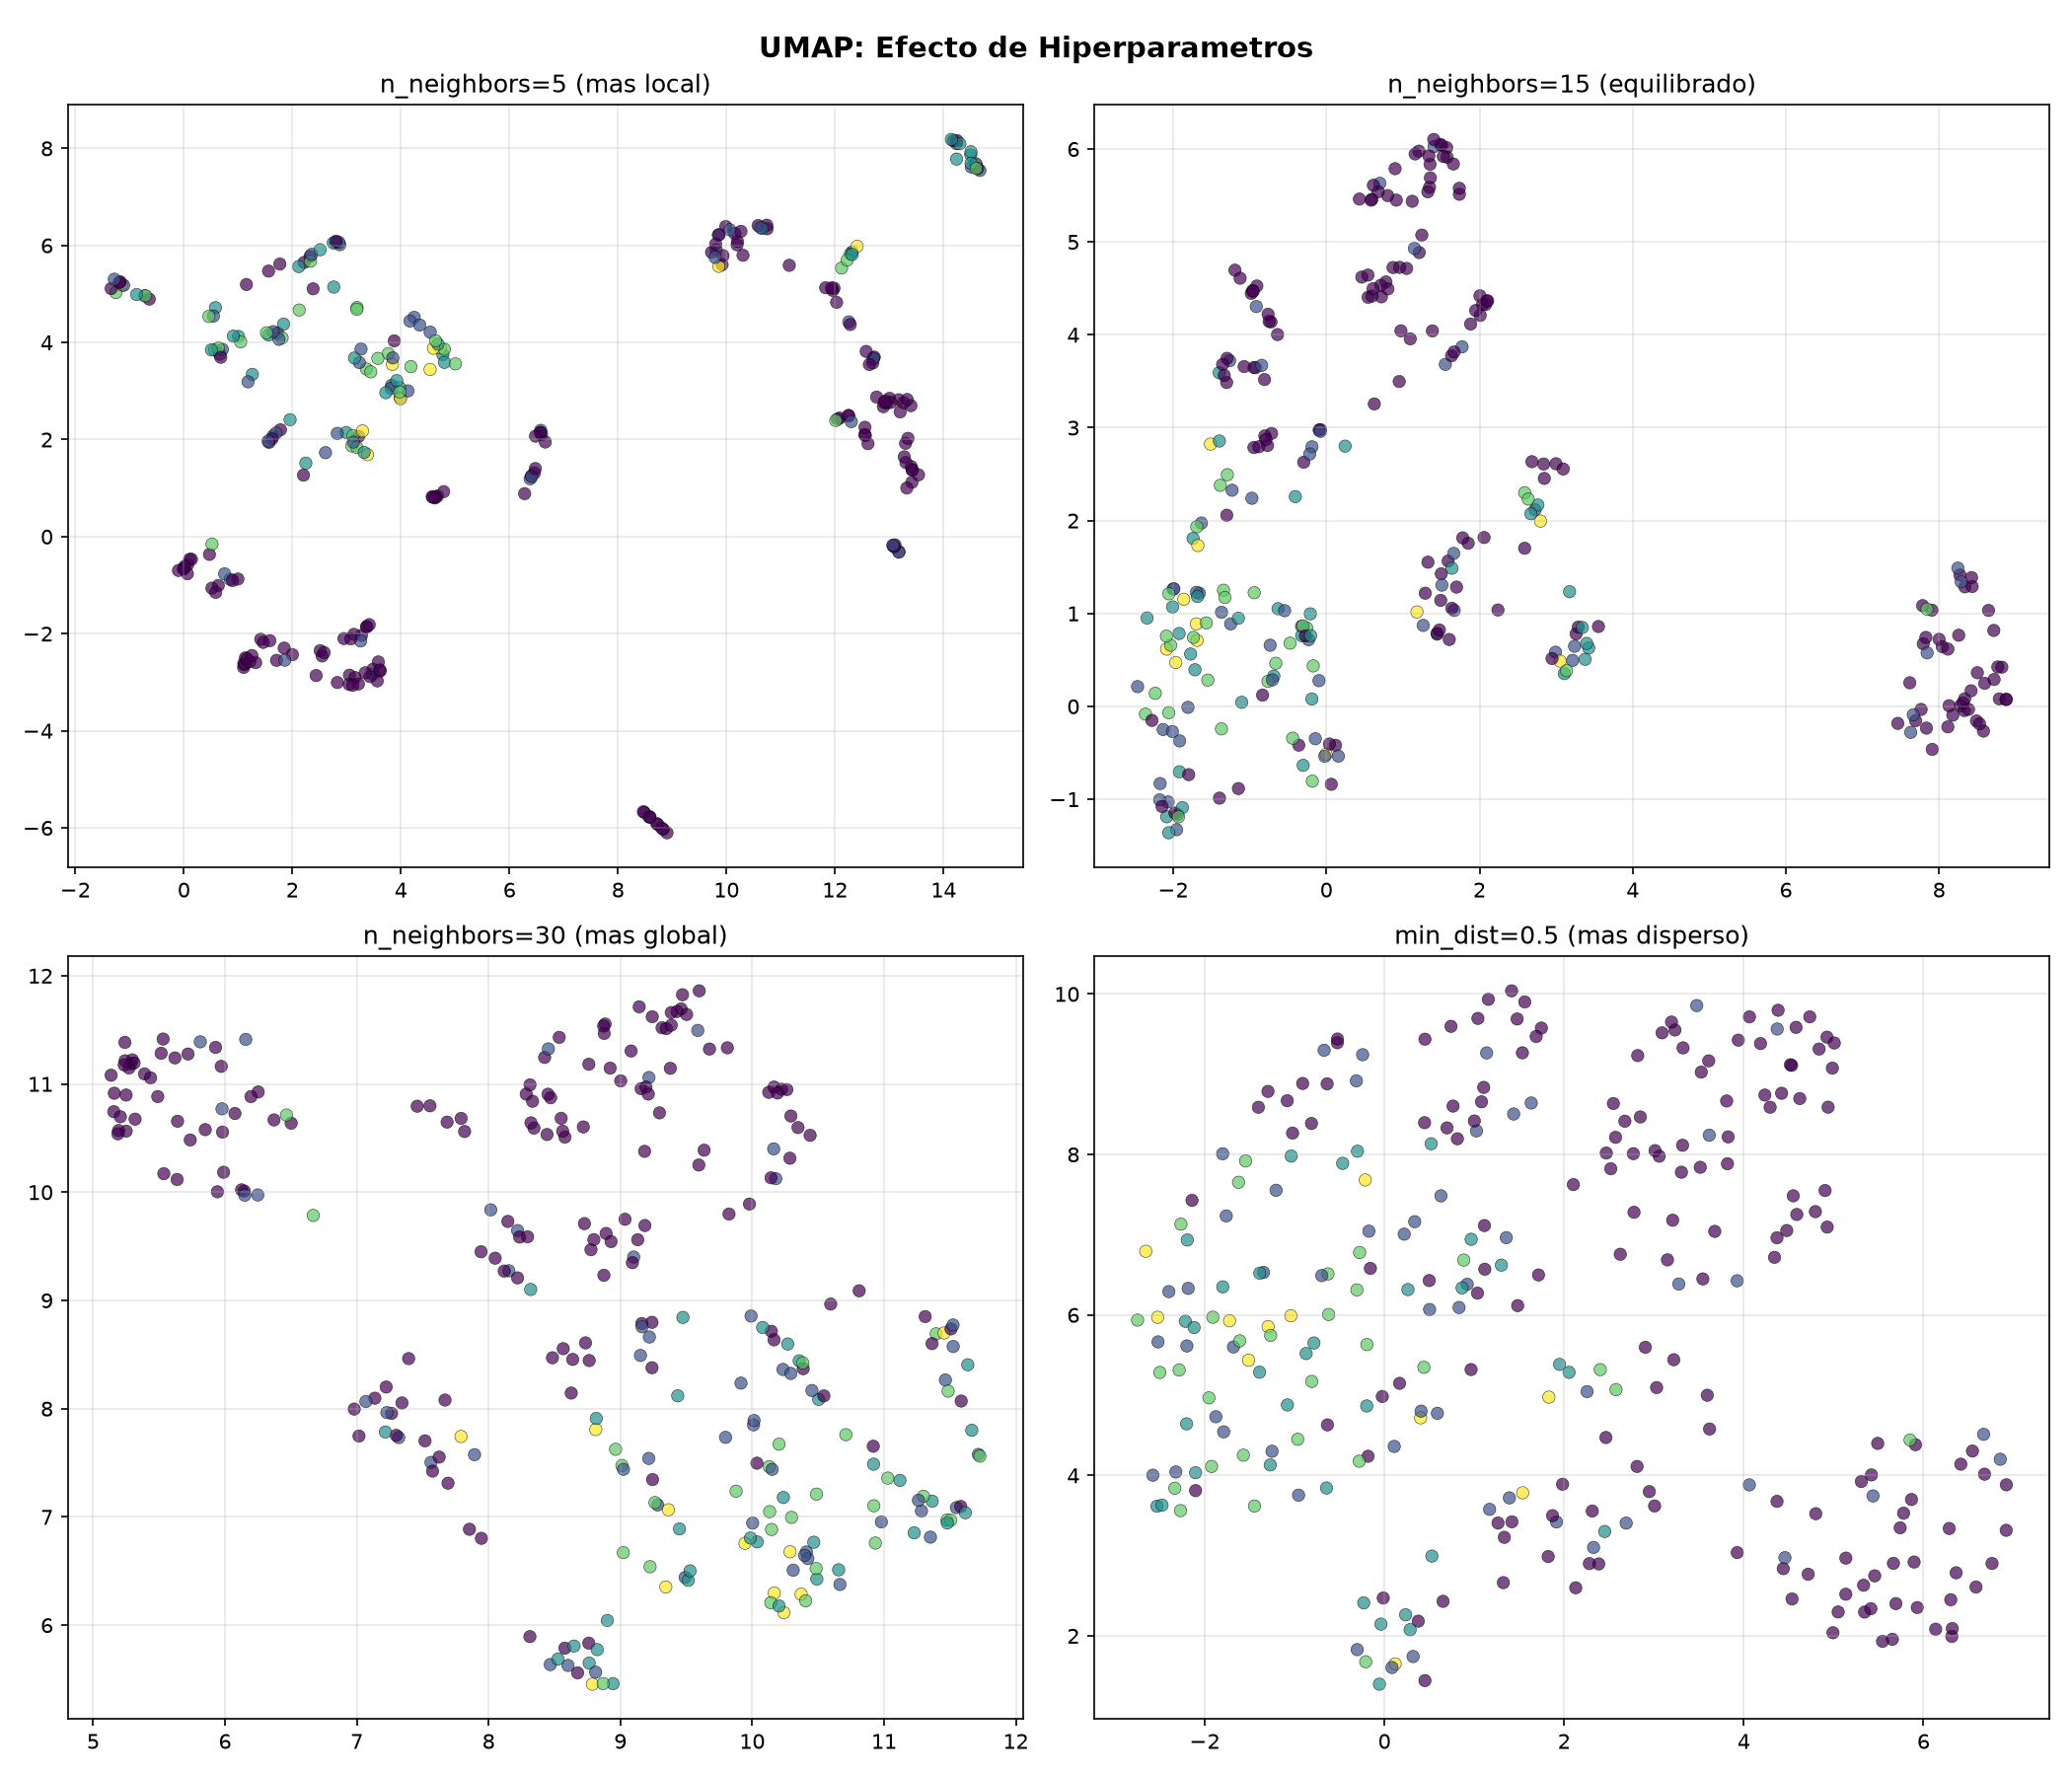
\includegraphics[height=0.65\textheight]{../plots/3_transformacion/umap_hiperparametros.png}
  \end{center}

  \begin{itemize}
    \item Exploración de \texttt{n\_neighbors} y \texttt{min\_dist} para balancear estructura local vs. global.
    \item Configuración final: \texttt{n\_neighbors=15}, \texttt{min\_dist=0.1}.
  \end{itemize}
\end{frame}

\begin{frame}{PCA vs. UMAP -- Comparación visual}
  \begin{center}
    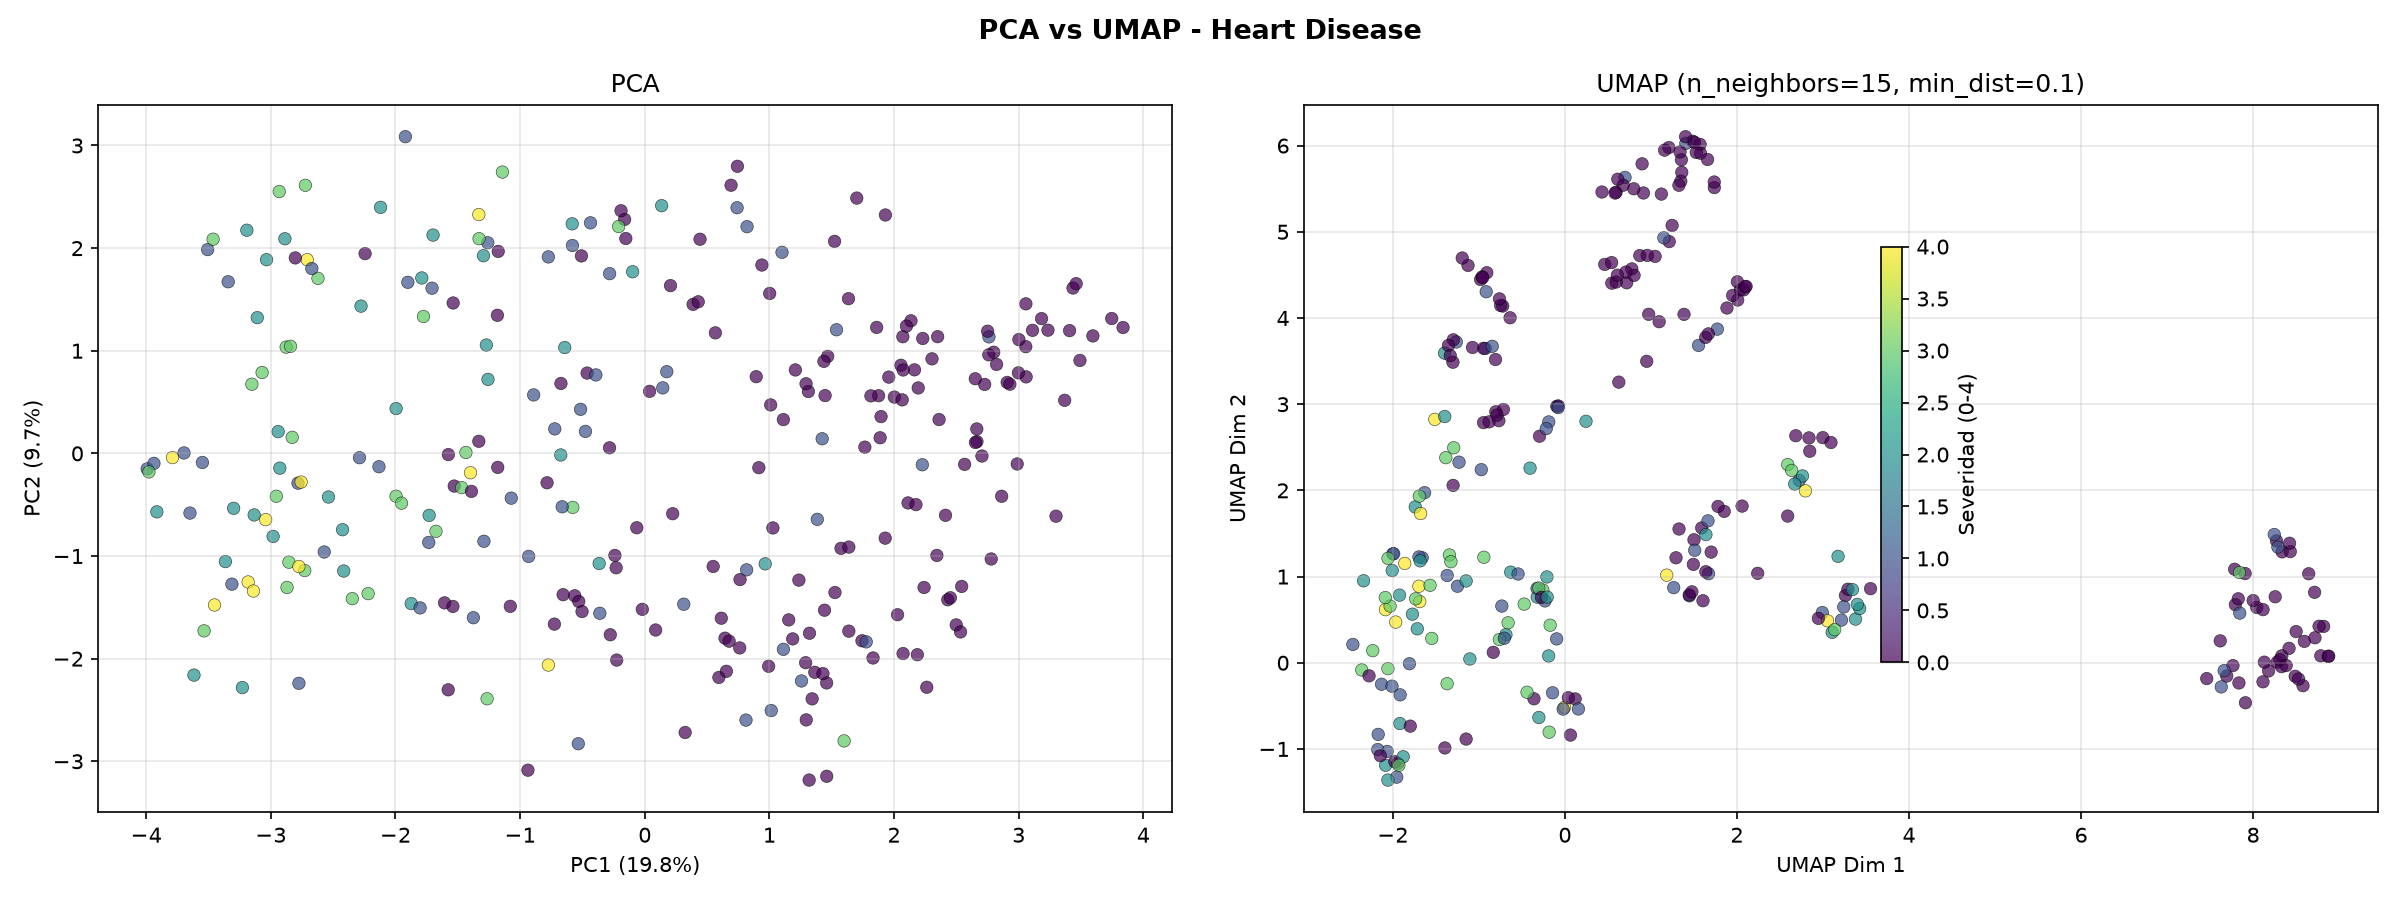
\includegraphics[height=0.60\textheight]{../plots/3_transformacion/pca_vs_umap.png}
  \end{center}

  \begin{itemize}
    \item \textbf{PCA} (izquierda): estructura global, poca separación entre clases.
    \item \textbf{UMAP} (derecha): revela subgrupos que PCA oculta; preserva mejor la topología local.
  \end{itemize}
\end{frame}

% ============================================================
% SECCIÓN 3: CLUSTERING
% ============================================================
\section{Clustering}

\begin{frame}{Clustering: dos enfoques complementarios}
  \textbf{K-Means} (particional):
  \begin{itemize}
    \item Asume clusters esféricos, isotrópicos y de tamaño similar.
    \item Requiere fijar $k$ a priori (método del codo + Silhouette).
    \item Eficiente; ideal para verificar si los perfiles clínicos forman grupos compactos.
  \end{itemize}

  \vspace{0.3cm}
  \textbf{OPTICS} (densidad):
  \begin{itemize}
    \item No requiere especificar $\varepsilon$ (a diferencia de DBSCAN).
    \item Maneja clusters de densidad variable y aísla ruido (perfiles atípicos).
    \item Produce un ordenamiento de puntos (reachability plot) que revela la estructura jerárquica de densidad.
  \end{itemize}

  \vspace{0.3cm}
  Ambos se aplican sobre las dos proyecciones 2D: \textbf{PCA} (EX1, EX2) y \textbf{UMAP} (EX3, EX4).
\end{frame}

\begin{frame}{OPTICS: Configuración utilizada}
  \begin{itemize}
    \item \texttt{min\_samples = 5}
    \item \texttt{xi = 0.05} (método de extracción de clusters)
    \item \texttt{max\_eps = $\infty$}
  \end{itemize}

  \vspace{0.3cm}
  Se aplicó OPTICS sobre dos proyecciones 2D: \textbf{PCA} y \textbf{UMAP}.
\end{frame}

\begin{frame}{OPTICS + PCA}
  \begin{center}
    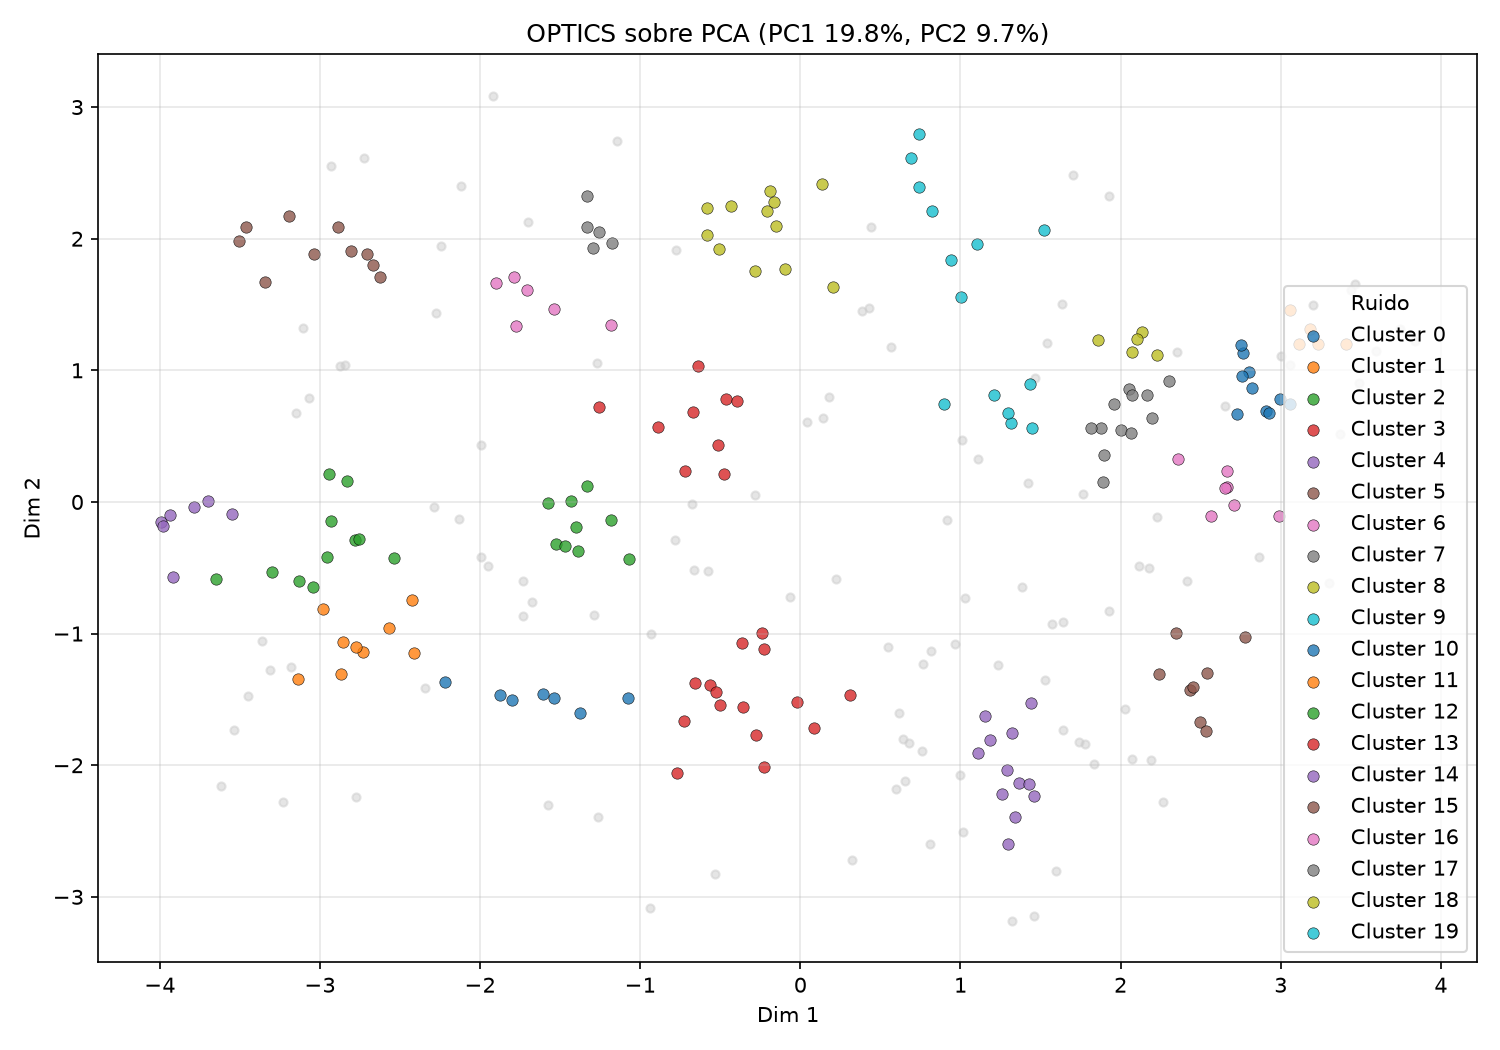
\includegraphics[height=0.60\textheight]{../plots/4_mineria/optics_pca.png}
  \end{center}

  \begin{itemize}
    \item Clusters detectados en el espacio PCA.
    \item El ruido (gris) se distribuye principalmente entre los grupos, en zonas de baja densidad.
  \end{itemize}
\end{frame}

\begin{frame}{OPTICS + UMAP}
  \begin{center}
    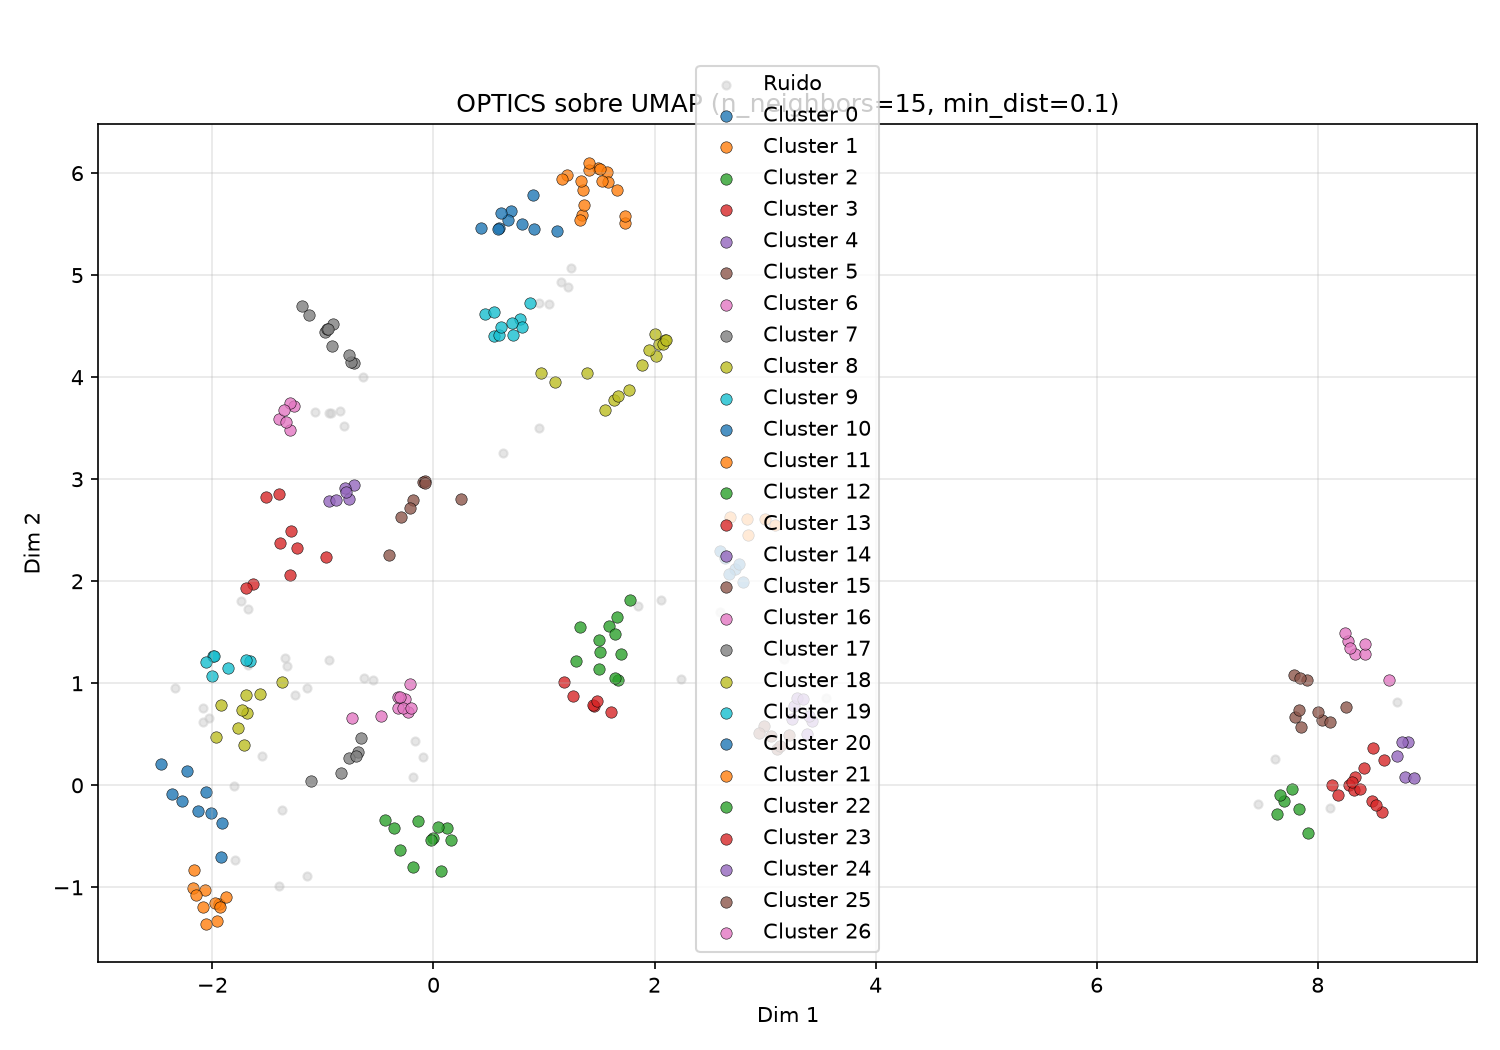
\includegraphics[height=0.60\textheight]{../plots/4_mineria/optics_umap.png}
  \end{center}

  \begin{itemize}
    \item UMAP revela grupos más compactos y mejor definidos que PCA.
    \item Menor proporción de ruido en comparación con la proyección lineal.
  \end{itemize}
\end{frame}

\begin{frame}{Reachability Plots}
  \begin{center}
    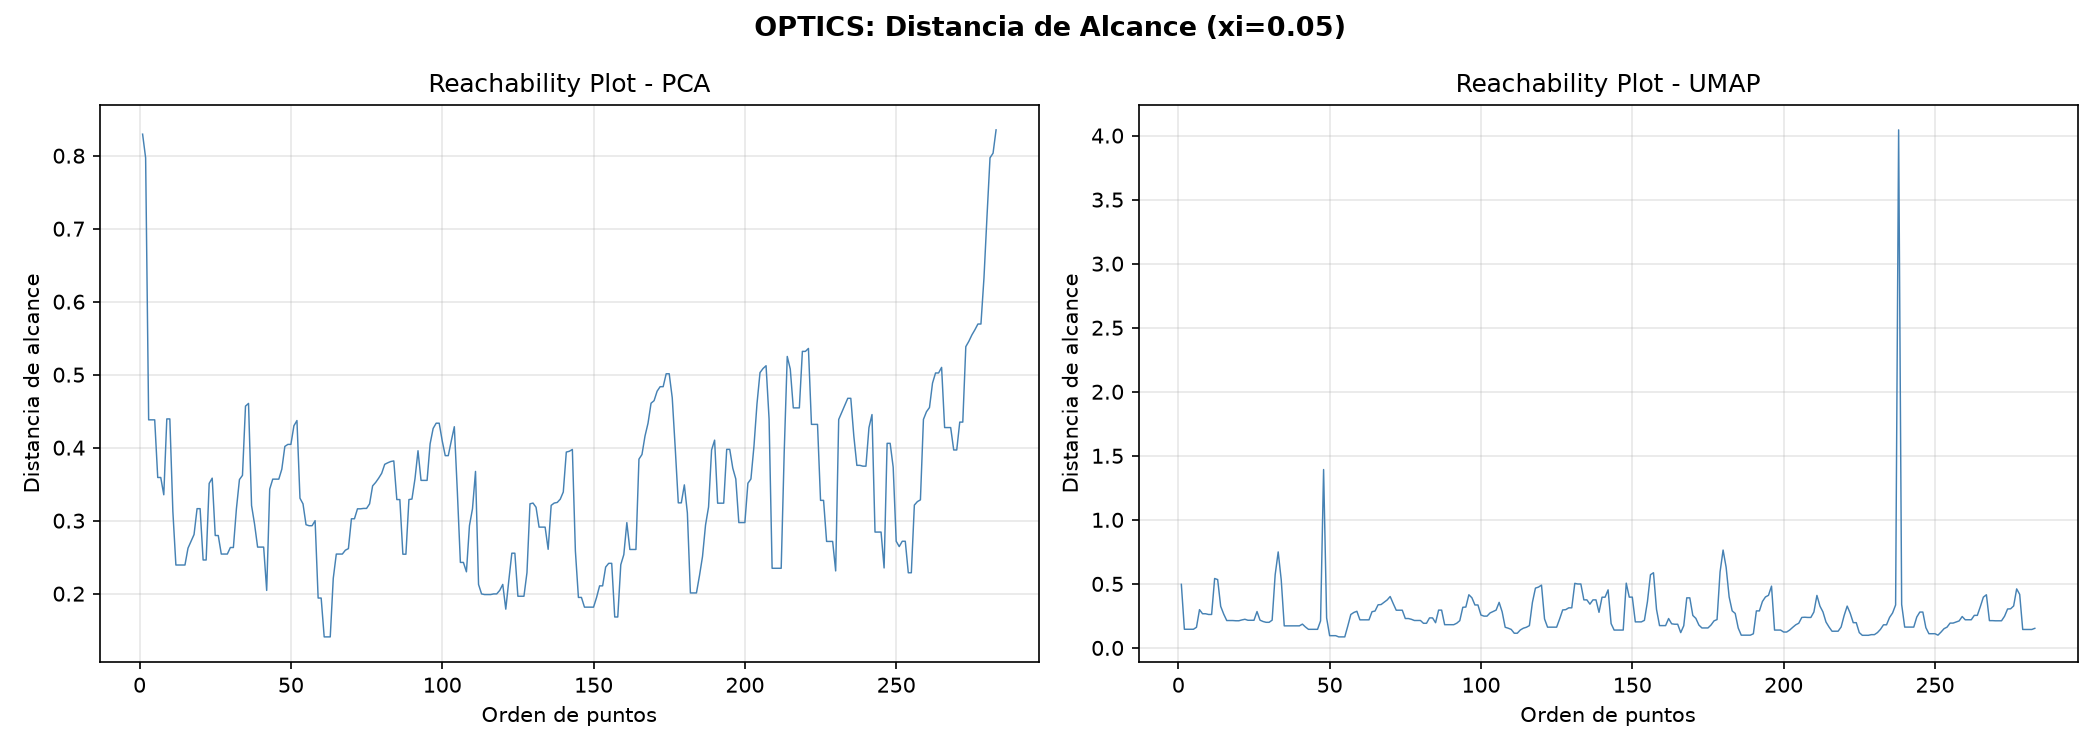
\includegraphics[height=0.60\textheight]{../plots/4_mineria/optics_reachability.png}
  \end{center}

  \begin{itemize}
    \item Los ``valles'' en el reachability plot indican clusters de alta densidad.
    \item UMAP (derecha) produce valles más pronunciados y definidos que PCA, lo que sugiere una estructura de densidad más clara.
  \end{itemize}
\end{frame}

\begin{frame}{K-Means: selección de $k$ (método del codo)}
  \begin{columns}
    \column{0.5\textwidth}
      \centering
      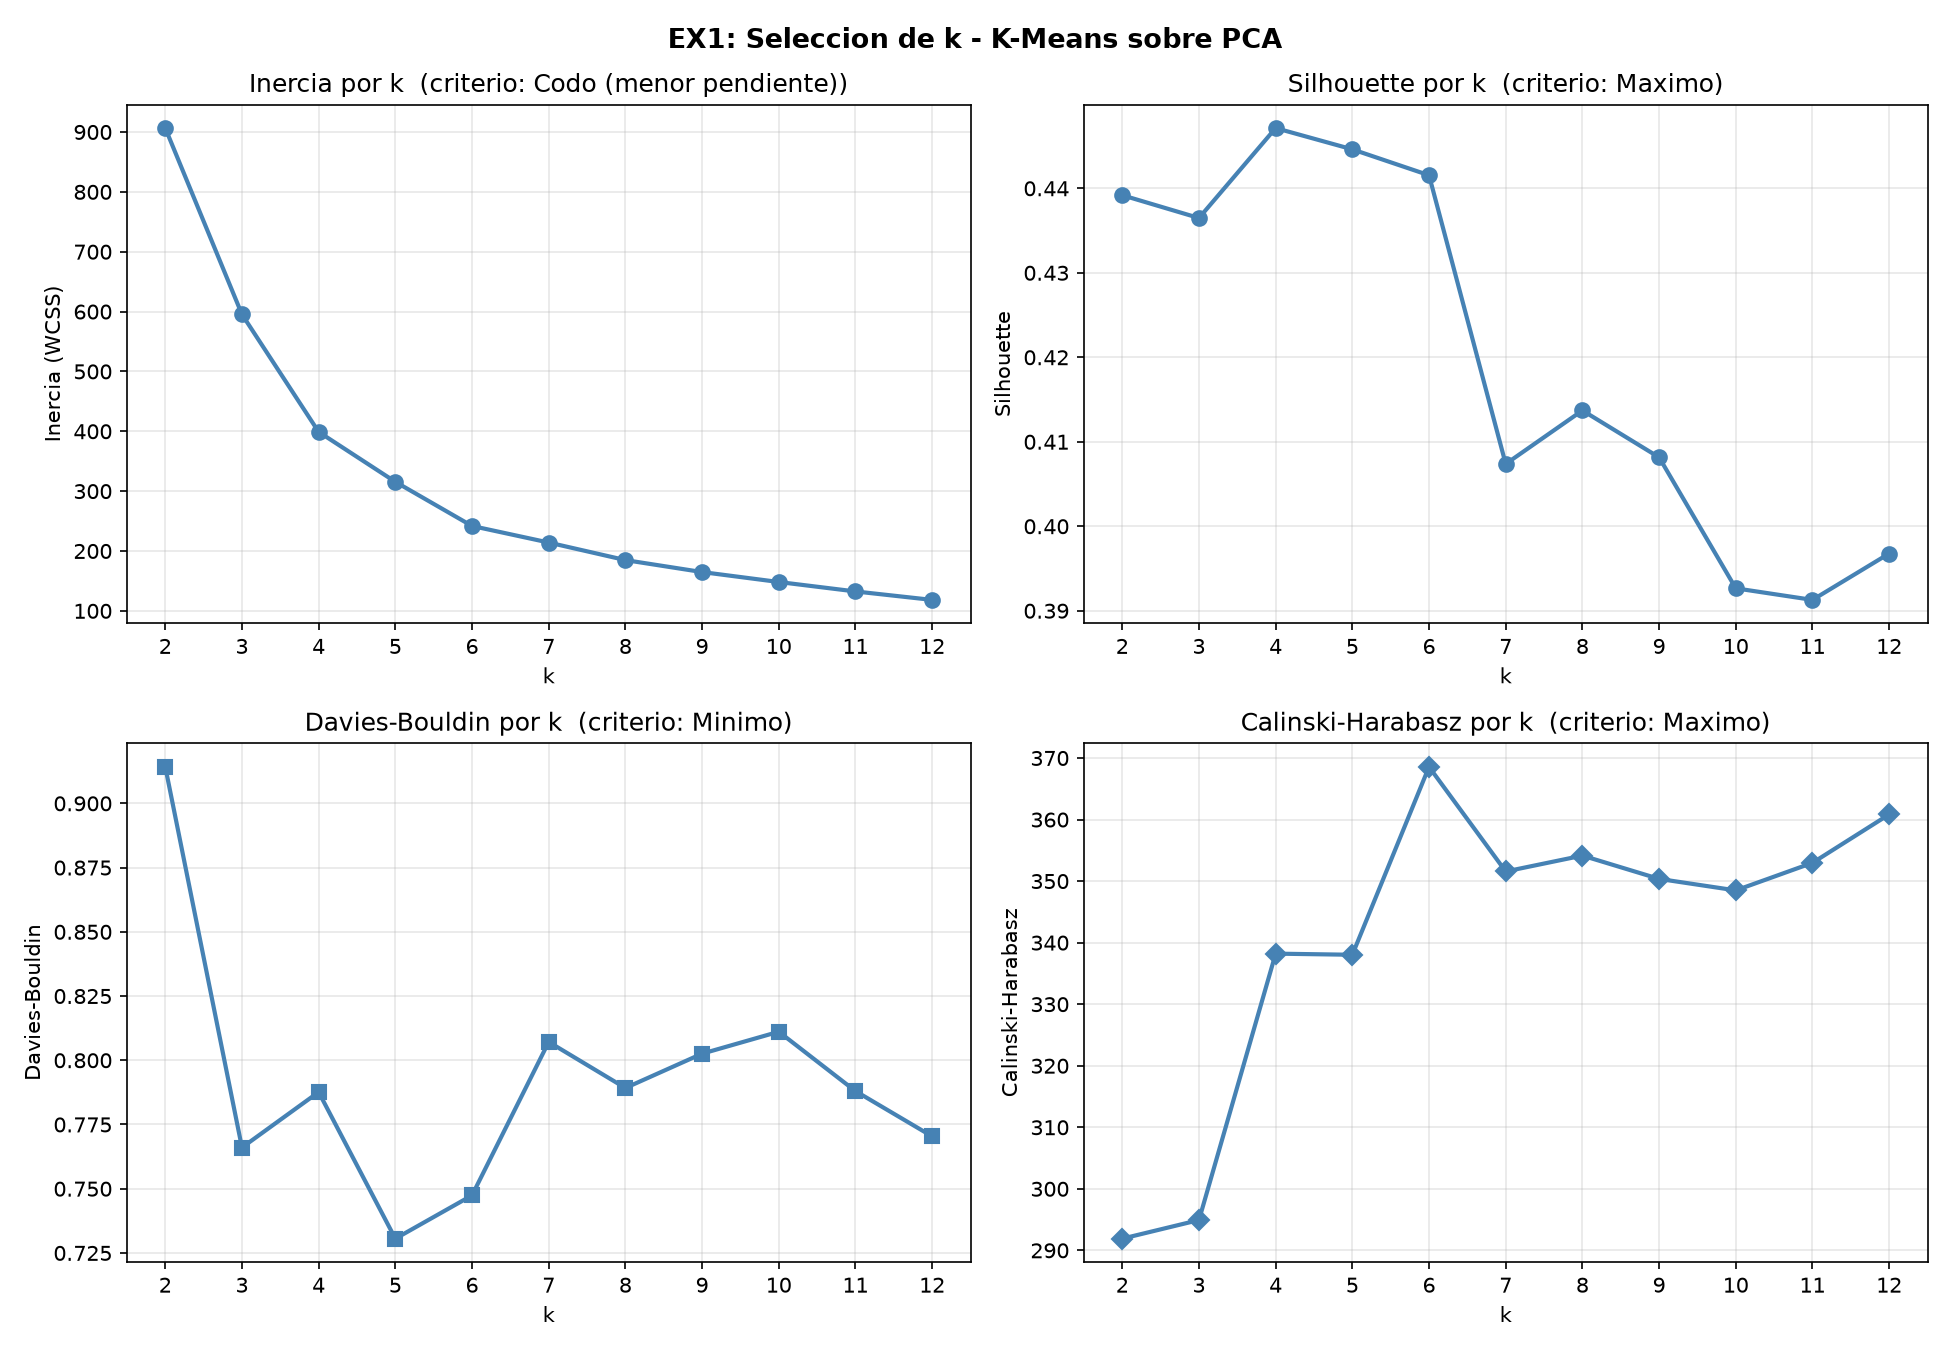
\includegraphics[width=\textwidth]{../plots/4_mineria/kmeans_codo_pca.png}
      \textbf{EX1: PCA + K-Means}

    \column{0.5\textwidth}
      \centering
      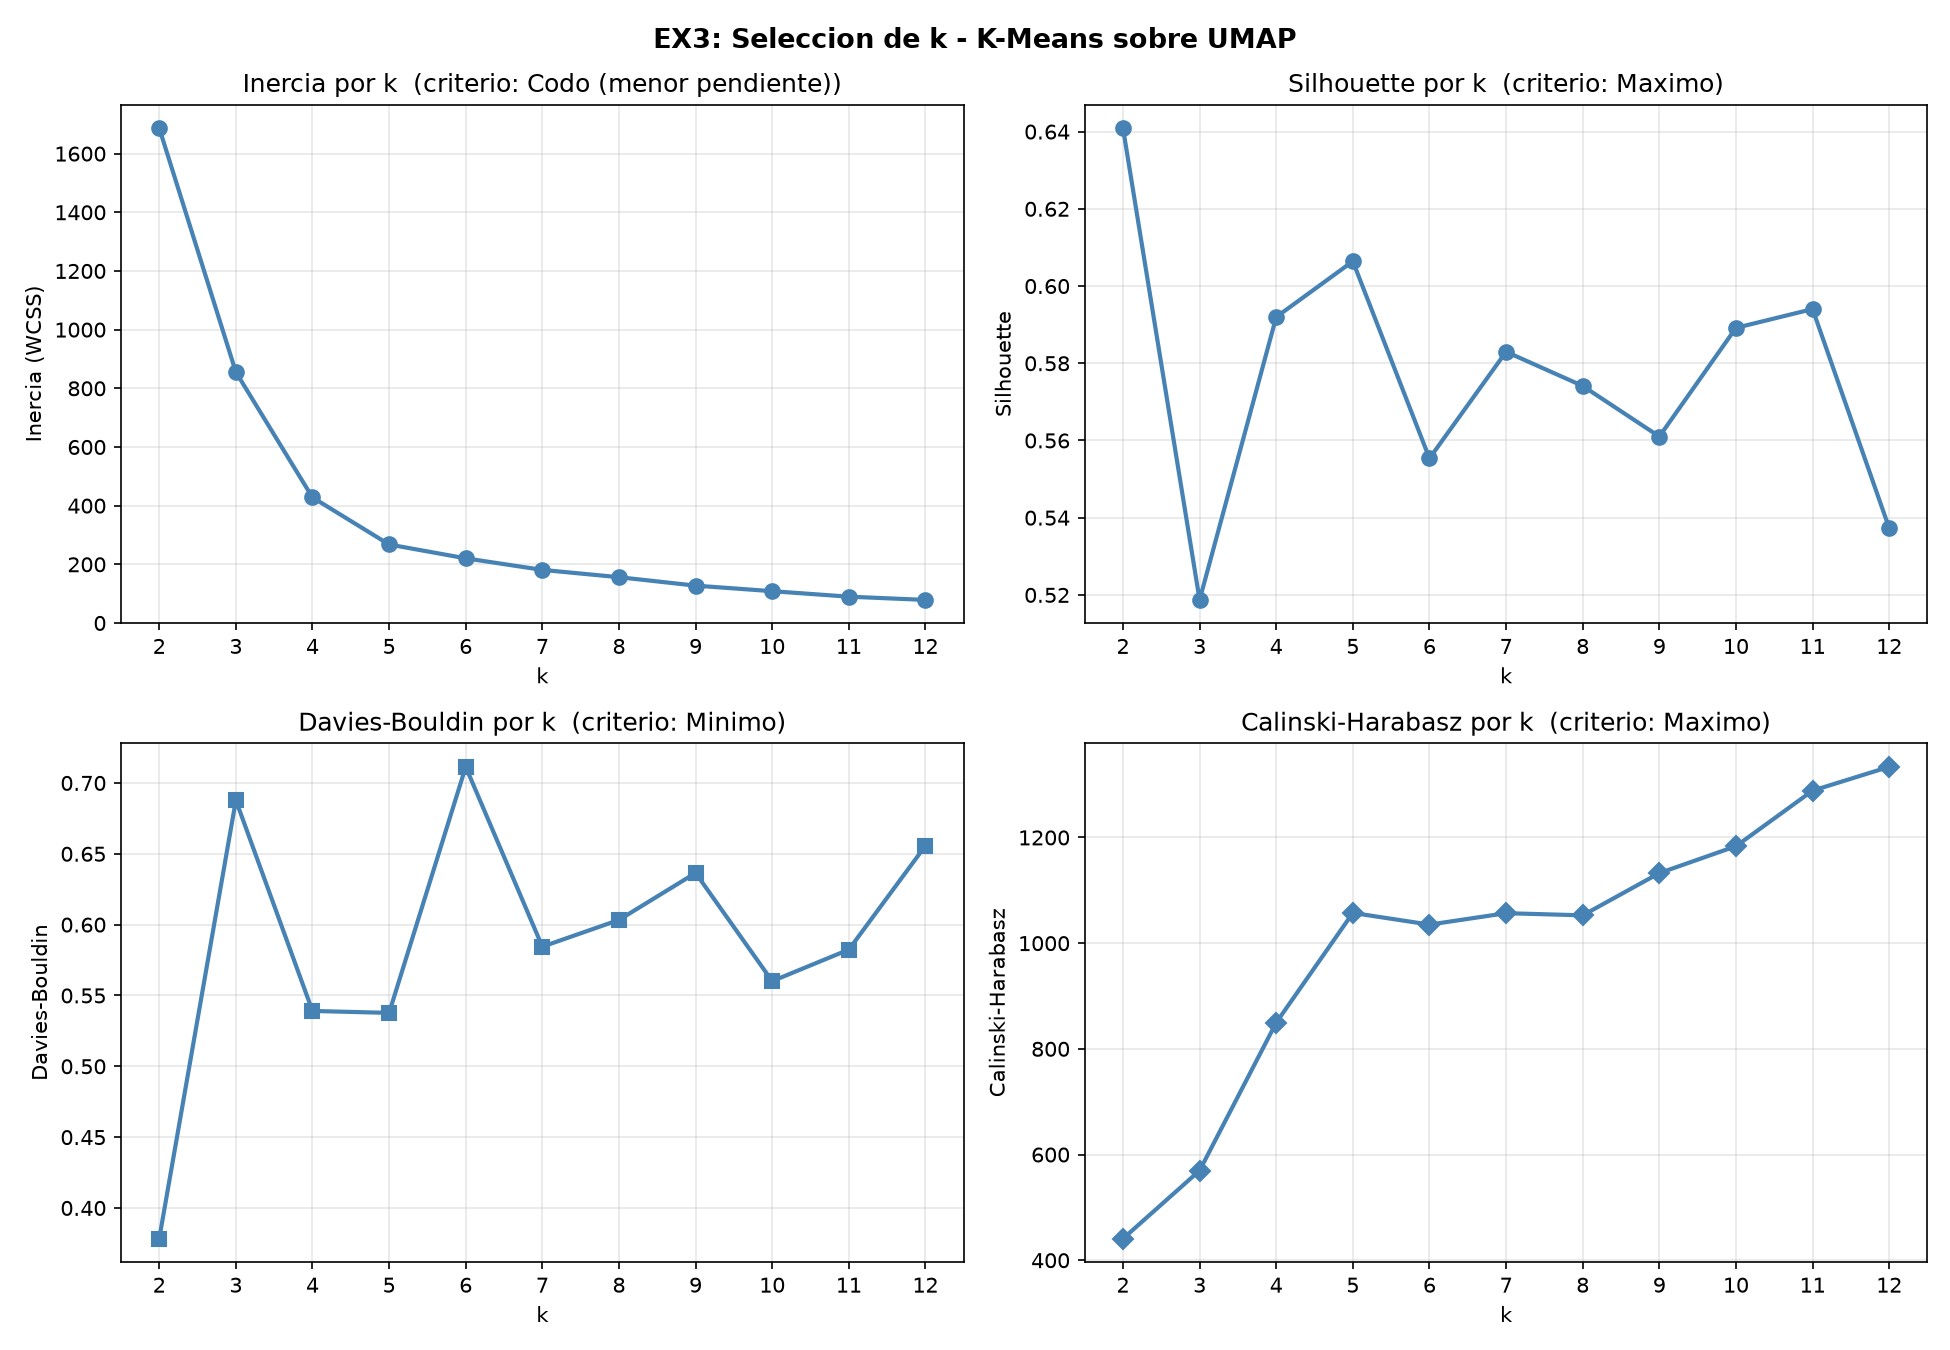
\includegraphics[width=\textwidth]{../plots/4_mineria/kmeans_codo_umap.png}
      \textbf{EX3: UMAP + K-Means}
  \end{columns}

  \vspace{0.2cm}
  \begin{itemize}
    \item El codo de la inercia sugiere $k \approx 4$--$5$ en ambas proyecciones.
    \item Criterios complementarios: \textbf{Silhouette} y \textbf{Davies-Bouldin} confirman el rango ($k=4$ en PCA, $k=2$ en UMAP).
  \end{itemize}
\end{frame}

\begin{frame}{K-Means: gráfico Silhouette ($k$ óptimo)}
  \begin{center}
    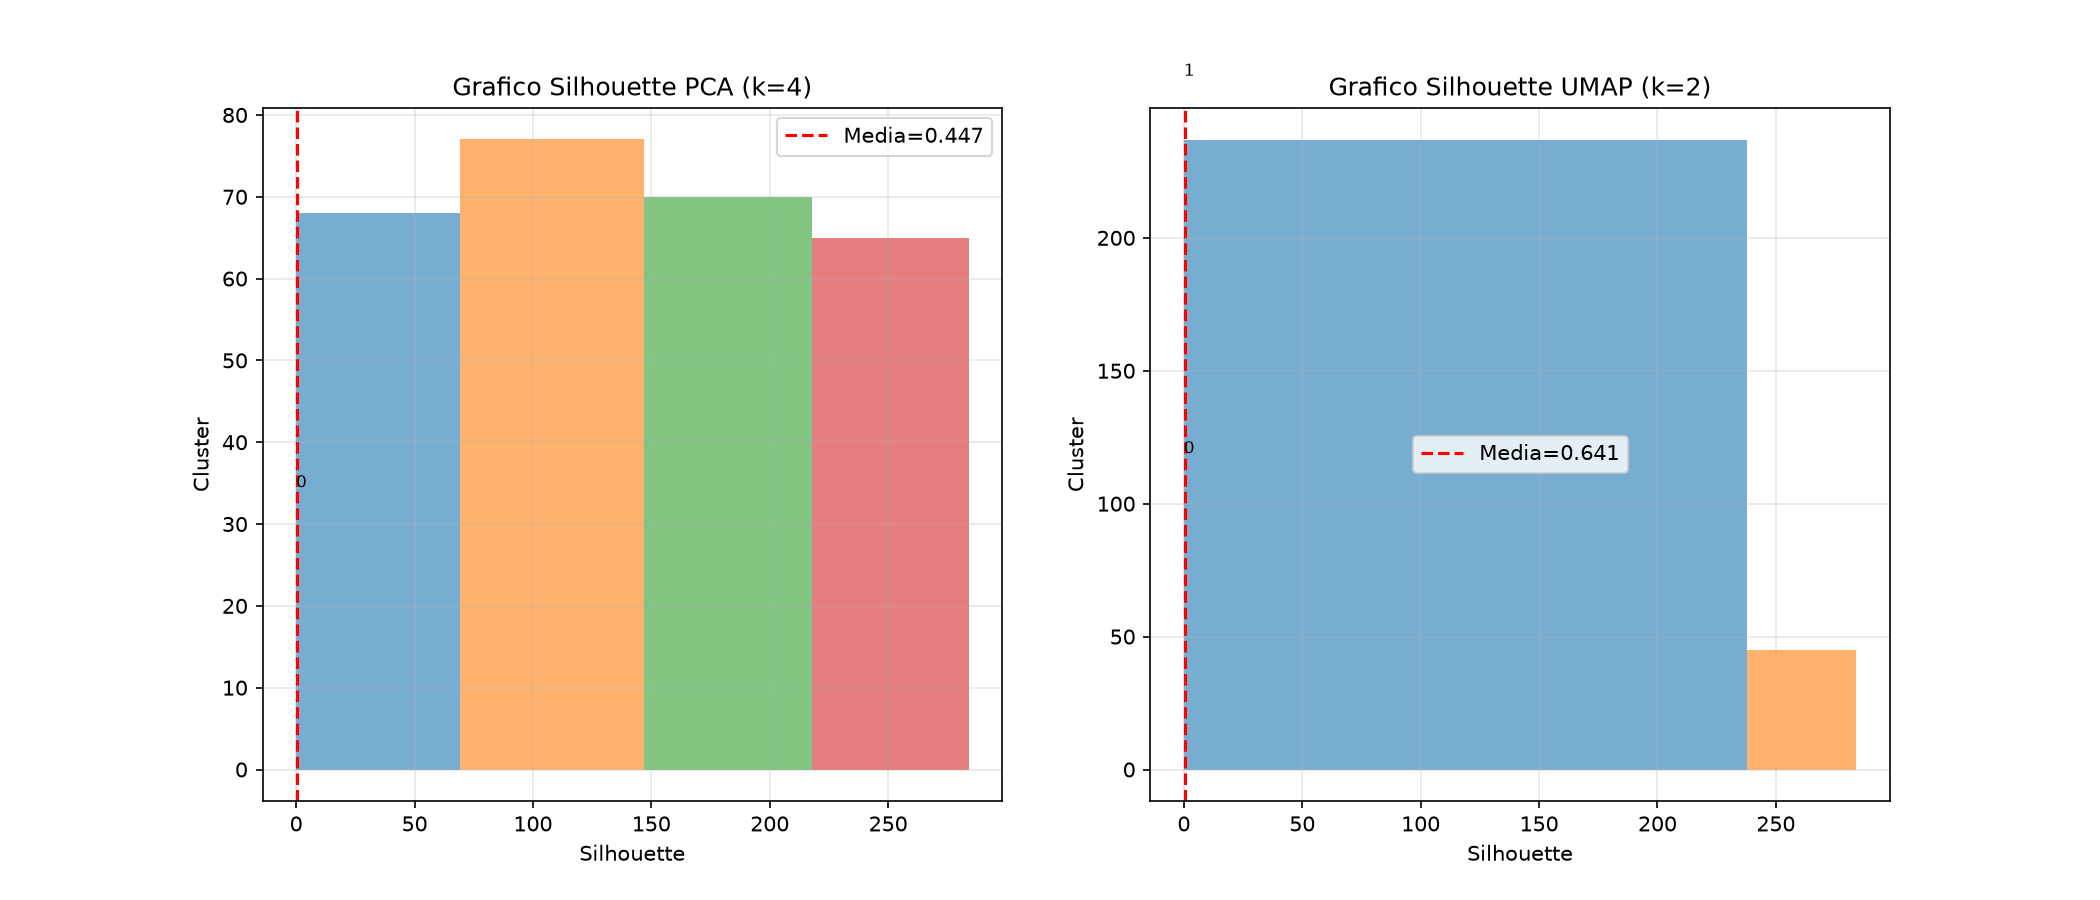
\includegraphics[height=0.60\textheight]{../plots/4_mineria/kmeans_silhouette.png}
  \end{center}

  \begin{itemize}
    \item \textbf{PCA ($k=4$):} Silhouette media 0.447, clusters de tamaño balanceado.
    \item \textbf{UMAP ($k=2$):} Silhouette media 0.641, clusters muy compactos y separados (coherente con la estructura no lineal).
  \end{itemize}
\end{frame}

\begin{frame}{EX1: K-Means sobre PCA ($k=4$)}
  \begin{center}
    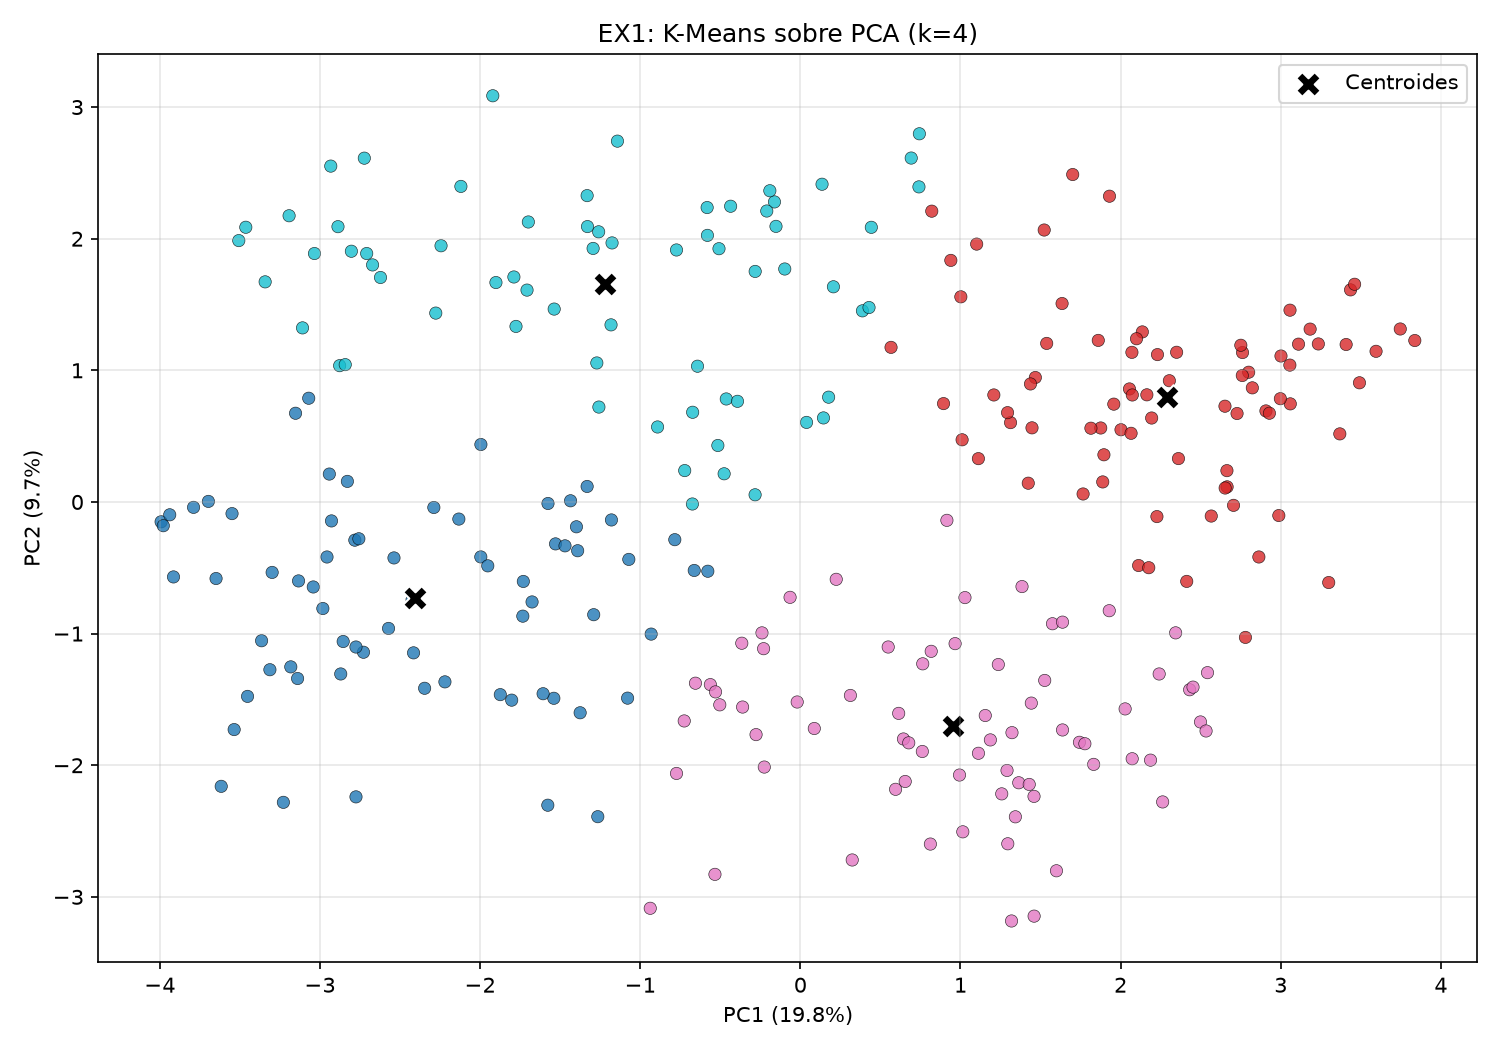
\includegraphics[height=0.60\textheight]{../plots/4_mineria/kmeans_pca.png}
  \end{center}

  \begin{itemize}
    \item \textbf{Cluster 1} (jóvenes, 49 años, thalach alto): 92\% de pacientes sanos.
    \item \textbf{Clusters 0 y 3} (oldpeak elevado, thalach bajo): mayor proporción de severidad 1--3.
    \item Los centroides (X) se reconstruyeron al espacio original para interpretar cada perfil.
  \end{itemize}
\end{frame}

\begin{frame}{EX3: K-Means sobre UMAP ($k=2$)}
  \begin{center}
    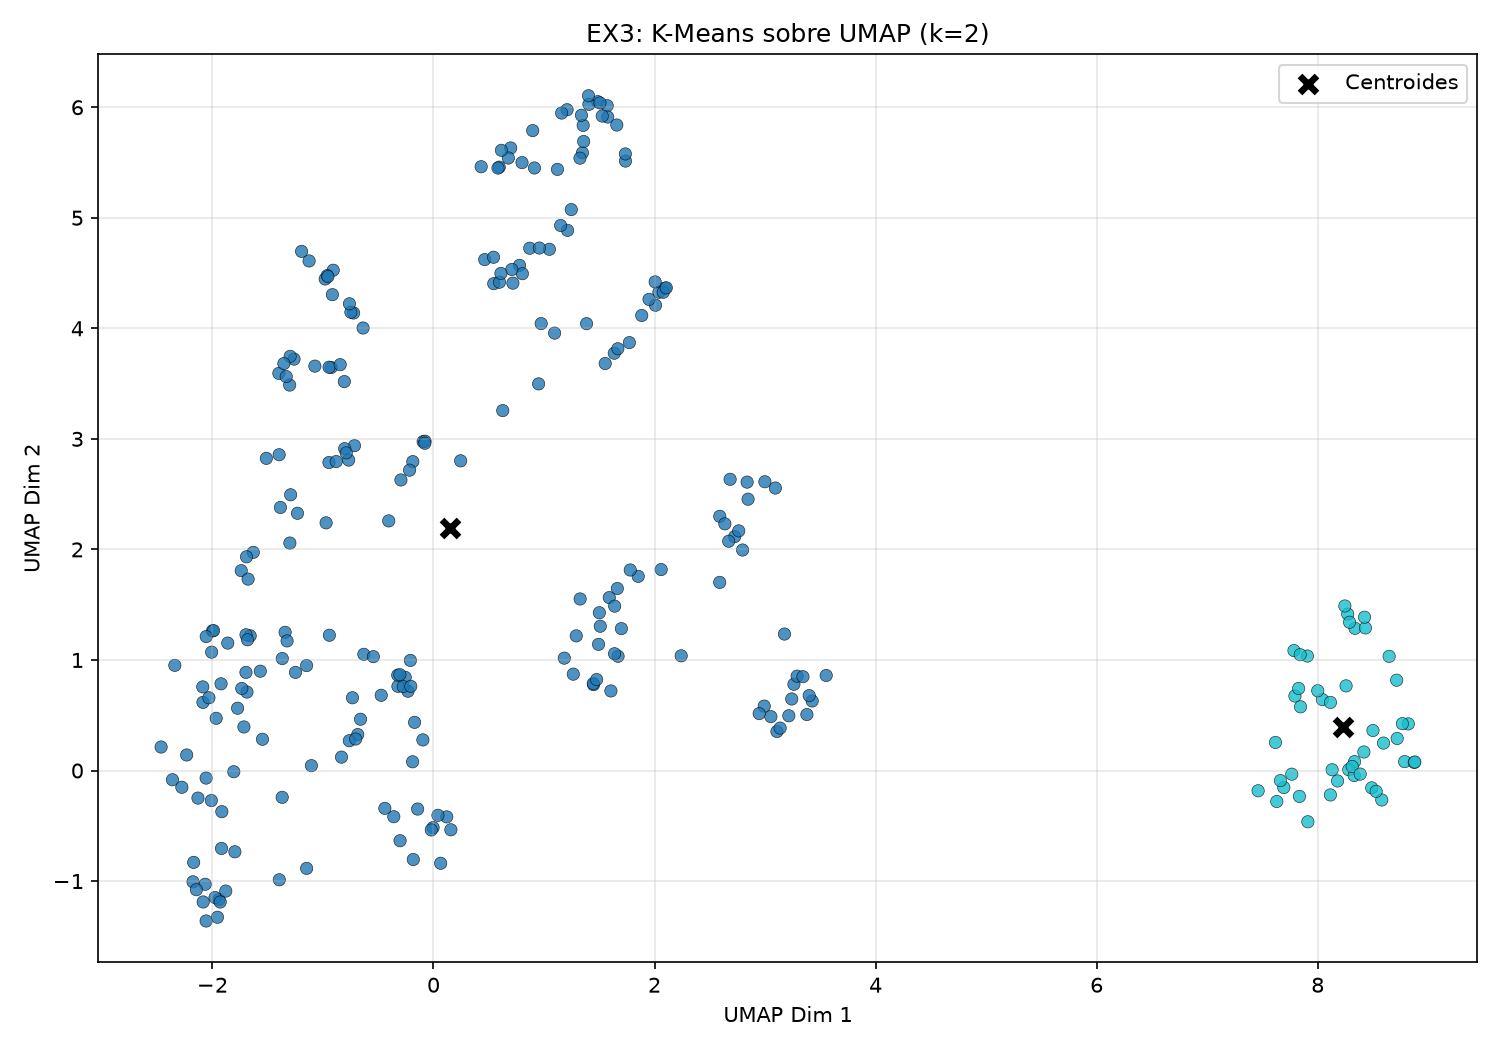
\includegraphics[height=0.60\textheight]{../plots/4_mineria/kmeans_umap.png}
  \end{center}

  \begin{itemize}
    \item La partición en 2 grupos (sano / enfermo, hipótesis inicial del plan) es la más compacta de todas ($\text{Silhouette} = 0.641$).
    \item Silhouette perfecta: los grupos no se traslapan en el espacio UMAP.
    \item Los clusters no coinciden con los 5 niveles de severidad (ARI $\approx 0$): agrupan por perfil clínico, no por etiqueta.
  \end{itemize}
\end{frame}

% ============================================================
% SECCIÓN 4: EVALUACIÓN Y MÉTRICAS
% ============================================================
\section{Evaluación y métricas}

\begin{frame}{Métricas de preservación topológica}
  \begin{center}
    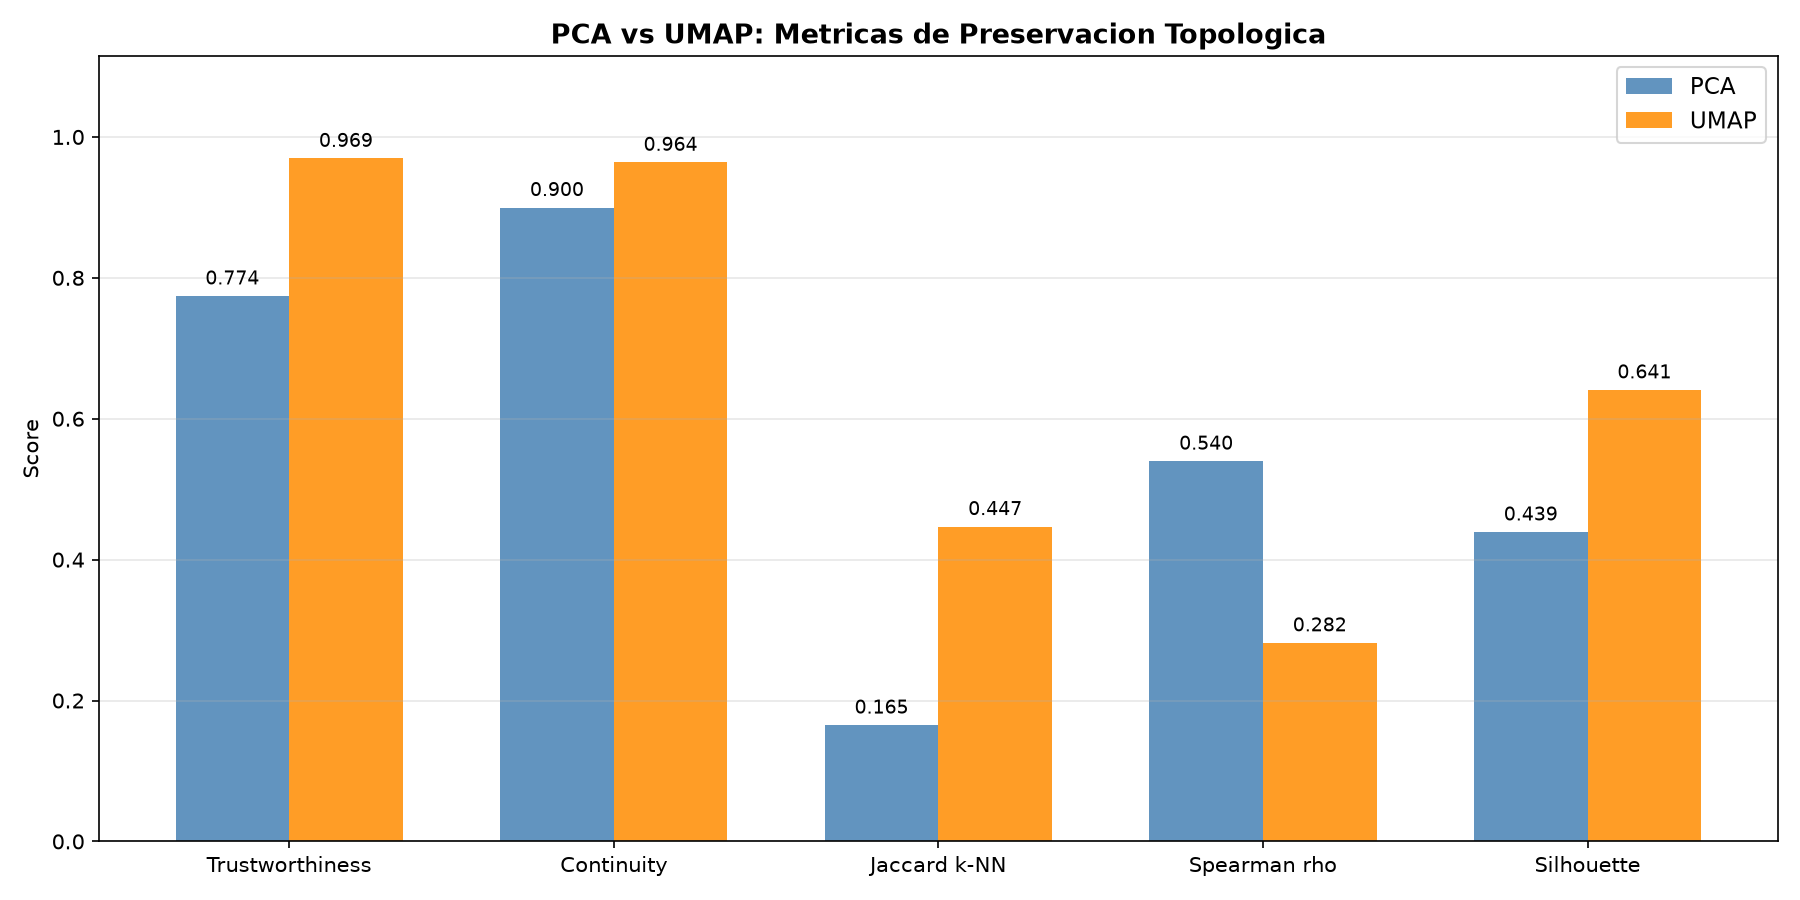
\includegraphics[height=0.60\textheight]{../plots/5_evaluacion/pca_vs_umap_metrics.png}
  \end{center}

  \textbf{Métricas calculadas:}
  \begin{itemize}
    \item \textbf{Trustworthiness:} ¿Cuán fiel es la vecindad en el espacio reducido?
    \item \textbf{Continuity:} ¿Se preservan todas las vecindades originales?
    \item \textbf{Jaccard k-NN:} Solapamiento de vecinos entre espacio original y reducido.
    \item \textbf{Spearman $\rho$:} Correlación de distancias.
    \item \textbf{Silhouette:} Cohesión y separación de clusters (KMeans, $k=2$).
  \end{itemize}
\end{frame}

\begin{frame}{Interpretación de métricas}
  \begin{block}{Resultados clave}
    \begin{itemize}
      \item \textbf{UMAP supera a PCA} en la mayoría de métricas de preservación topológica.
      \item \textbf{Trustworthiness y Jaccard:} UMAP preserva mejor las vecindades originales.
      \item \textbf{Silhouette:} UMAP produce estructuras más compactas y separables.
      \item \textbf{Spearman $\rho$:} PCA mantiene mejor la correlación global de distancias (ventaja lineal esperada).
    \end{itemize}
  \end{block}

  \vspace{0.3cm}
  \textbf{Conclusión:} Para este dataset con estructura no lineal, UMAP es superior como paso previo al clustering.
\end{frame}

\begin{frame}{Resultados del clustering (EX1--EX4)}
  \begin{center}
    \small
    \begin{tabular}{lcccccc}
      \toprule
      \textbf{Modelo} & \textbf{k / cl.} & \textbf{Silhouette} & \textbf{Davies-Bouldin} & \textbf{Calinski-Harabasz} & \textbf{ARI} & \textbf{NMI} \\
      \midrule
      K-Means PCA   & 4  & 0.447 & 0.788 & 338.2  & 0.177 & 0.219 \\
      K-Means UMAP  & 2  & \textbf{0.641} & \textbf{0.378} & 440.8  & $-0.086$ & 0.064 \\
      OPTICS PCA    & 20 & 0.546 & 0.568 & 506.9  & 0.038 & 0.223 \\
      OPTICS UMAP   & 27 & 0.567 & 0.552 & \textbf{2194.1} & 0.036 & 0.207 \\
      \bottomrule
    \end{tabular}
  \end{center}

  \vspace{0.2cm}
  \begin{itemize}
    \item \textbf{K-Means + UMAP} ($k=2$) maximiza Silhouette y minimiza Davies-Bouldin: clusters compactos y separados.
    \item \textbf{OPTICS + UMAP} detecta 27 grupos densos (16.5\% de ruido) con la mayor Calinski-Harabasz.
    \item El \textbf{ARI/NMI bajo} en todos los modelos indica que los clusters agrupan por perfil clínico y no por el nivel de severidad etiquetado.
  \end{itemize}
\end{frame}

\begin{frame}{Comparación visual de métricas}
  \begin{center}
    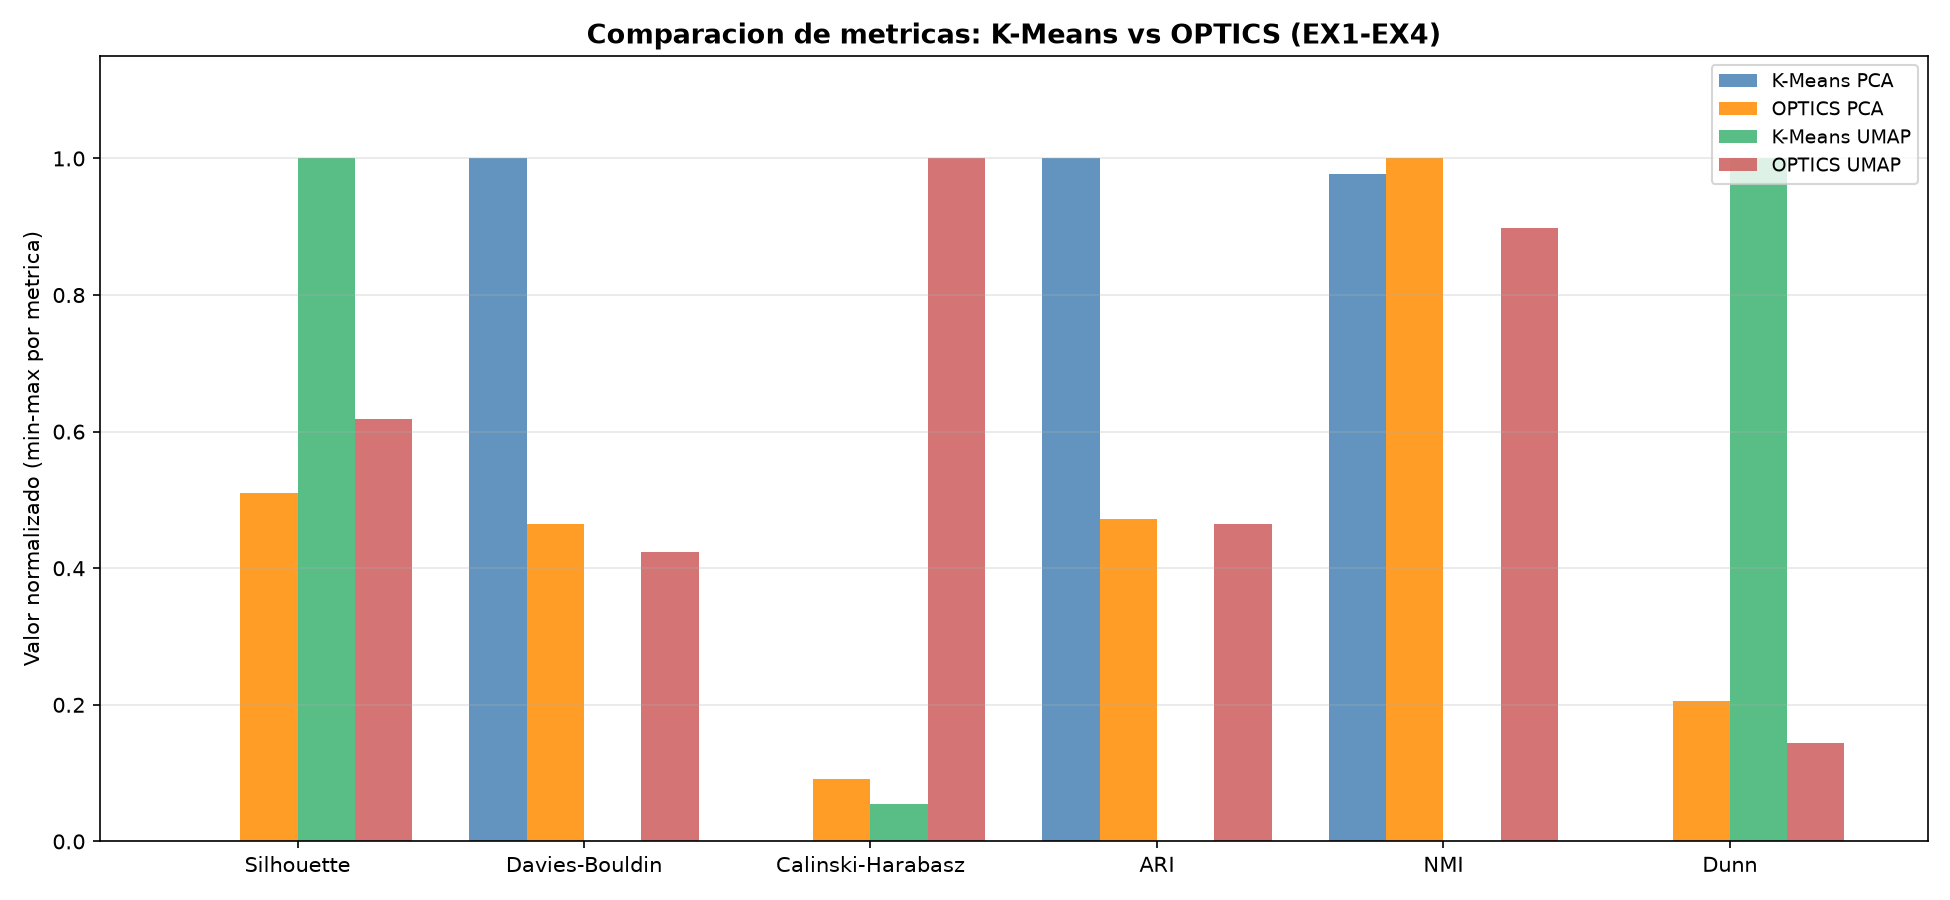
\includegraphics[height=0.55\textheight]{../plots/5_evaluacion/clustering_metrics.png}
  \end{center}

  \begin{itemize}
    \item Valores normalizados (min-max por métrica) para comparar escalas distintas.
    \item \textbf{K-Means UMAP} domina en las métricas intrínsecas de compactidad (Silhouette, Davies-Bouldin, Dunn).
    \item \textbf{OPTICS UMAP} domina en Calinski-Harabasz (separación global) por su alta cantidad de clusters.
    \item El ruido de OPTICS (39.1\% en PCA) degrada su utilidad en la proyección lineal.
  \end{itemize}
\end{frame}

% ============================================================
% SECCIÓN 5: VISUALIZACIONES
% ============================================================
\section{Visualizaciones}

\begin{frame}{Resumen visual del flujo de trabajo}
  \begin{enumerate}
    \item \textbf{EDA:} Histogramas, boxplots y heatmap de correlación para entender la distribución y relaciones entre variables.
    \item \textbf{Preprocesamiento:} Comparativa antes/después de eliminación de outliers.
    \item \textbf{Reducción:} Scree plot, loadings, proyecciones 2D (PCA y UMAP).
    \item \textbf{Clustering:} Visualización de clusters K-Means (EX1, EX3) y OPTICS (EX2, EX4) sobre PCA y UMAP, reachability plots.
    \item \textbf{Evaluación:} Barras comparativas de métricas PCA vs. UMAP.
  \end{enumerate}

  \vspace{0.3cm}
  \begin{center}
    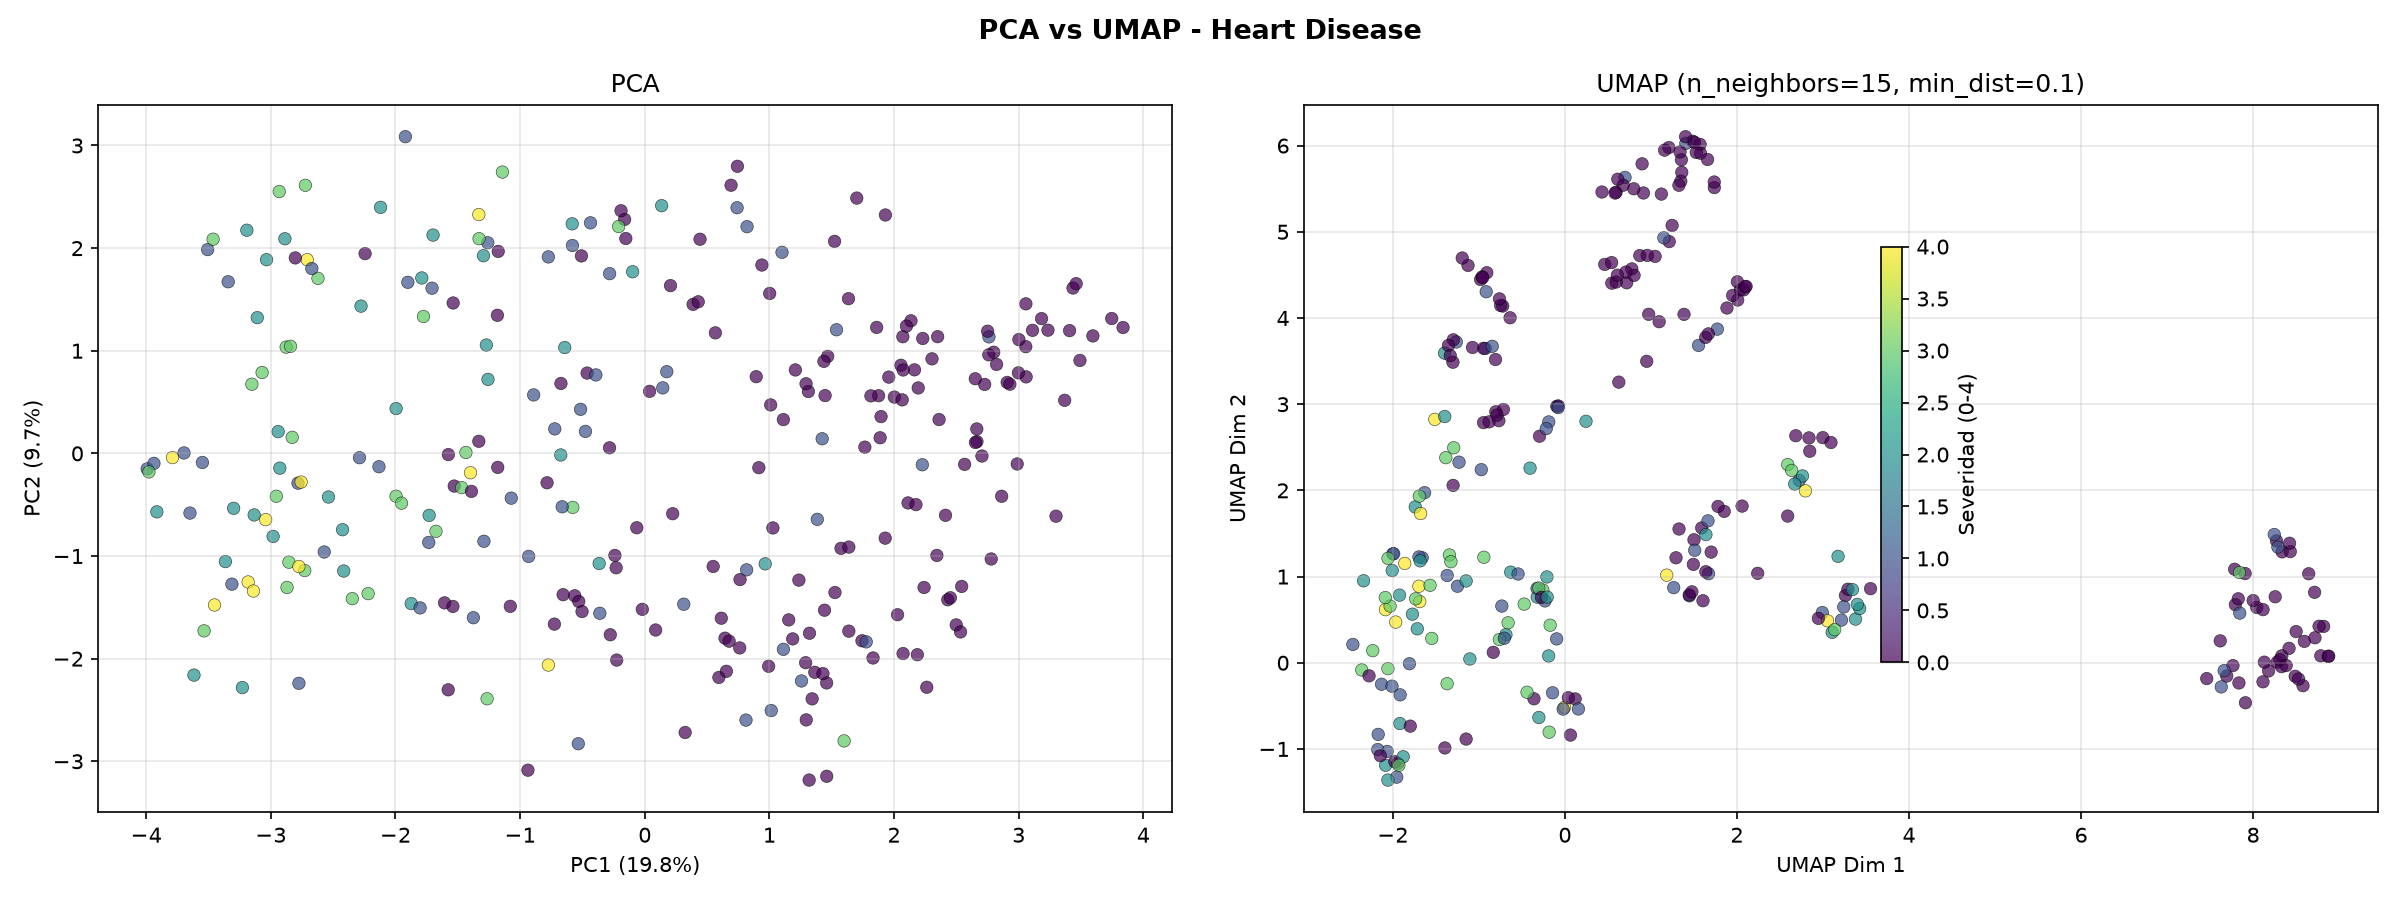
\includegraphics[height=0.30\textheight]{../plots/3_transformacion/pca_vs_umap.png}
    \hspace{0.3cm}
    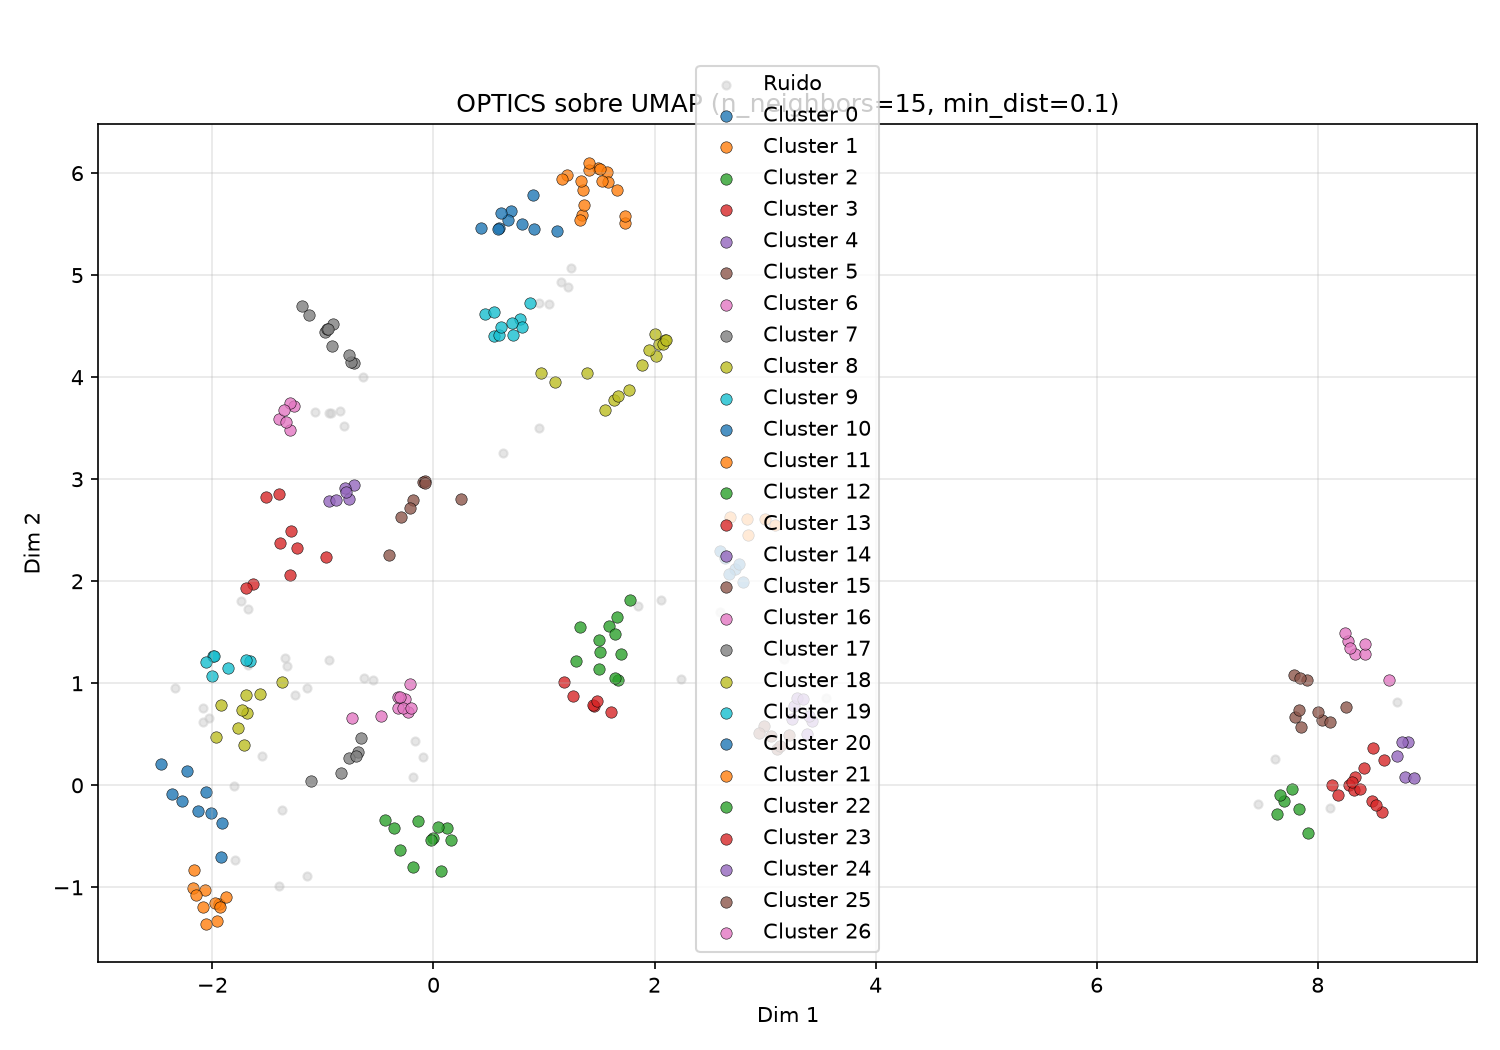
\includegraphics[height=0.30\textheight]{../plots/4_mineria/optics_umap.png}
  \end{center}
\end{frame}

% ============================================================
% SECCIÓN 6: INTERPRETACIÓN CRÍTICA
% ============================================================
\section{Interpretación crítica}

\begin{frame}{Interpretación crítica del análisis}
  \textbf{Fortalezas:}
  \begin{itemize}
    \item El pipeline de preprocesamiento es completo: imputación, codificación, detección de outliers y estandarización.
    \item La comparación PCA vs. UMAP es objetiva, respaldada por 5 métricas cuantitativas.
    \item OPTICS es una elección metodológica sólida para datasets con densidad variable.
  \end{itemize}

  \vspace{0.3cm}
  \textbf{Limitaciones:}
  \begin{itemize}
    \item \textbf{Dimensionalidad:} Con solo $\approx 29.5\%$ de varianza en 2D, PCA pierde mucha información. Se usó 2D por visualización, no por optimalidad.
    \item \textbf{Tamaño muestral:} 284 registros es limitado para clustering basado en densidad.
    \item \textbf{UMAP es estocástico:} Los resultados pueden variar entre ejecuciones si no se fija \texttt{random\_state}.
    \item \textbf{Validación externa débil:} ARI/NMI bajos en todos los modelos: los clusters no replican las etiquetas de severidad (0--4), que además no definen clases ``naturales'' bien separadas.
  \end{itemize}
\end{frame}

\begin{frame}{Lecciones aprendidas}
  \begin{itemize}
    \item La estructura no lineal del dataset (requiere 12 PCs para el 80\% de varianza) justifica plenamente el uso de UMAP.
    \item El preprocesamiento (outliers + escalado) tiene un impacto directo en la calidad de las proyecciones.
    \item Las métricas de preservación topológica son complementarias: una sola métrica no basta para decidir entre técnicas de reducción.
    \item \textbf{K-Means} y \textbf{OPTICS} sobre UMAP superan a sus versiones sobre PCA: el espacio no lineal revela grupos más compactos.
    \item La baja concordancia con el target (ARI/NMI) sugiere que la severidad 0--4 no forma grupos geométricamente ``naturales''.
  \end{itemize}

  \vspace{0.3cm}
  \begin{block}{Trabajo futuro}
    \begin{itemize}
      \item Explorar $n=3$ componentes en PCA/UMAP para reducir pérdida de información.
      \item Refinar la validación externa binaria (sano vs. enfermo) en lugar de los 5 niveles de severidad.
      \item Probar t-SNE y GMM (modelos de mezcla) como alternativas a UMAP y K-Means.
    \end{itemize}
  \end{block}
\end{frame}

% ============================================================
% SECCIÓN 7: CALIDAD
% ============================================================
\section{Calidad}

\begin{frame}{Evaluación de la calidad del análisis}
  \textbf{Calidad de los datos:}
  \begin{itemize}
    \item Solo 6 valores nulos en 303 registros (1.98\%) -- dataset de alta completitud.
    \item 19 outliers detectados y eliminados (6.3\% de las filas) con criterio IQR justificado.
    \item Estandarización verificada ($\mu \approx 0$, $\sigma \approx 1$).
  \end{itemize}

  \vspace{0.3cm}
  \textbf{Calidad de la reducción dimensional:}
  \begin{itemize}
    \item PCA: scree plot y varianza acumulada documentados. Loadings interpretados.
    \item UMAP: hiperparámetros explorados y justificados.
    \item Comparación objetiva con 5 métricas independientes.
  \end{itemize}

  \vspace{0.3cm}
  \textbf{Calidad del clustering:}
  \begin{itemize}
    \item K-Means: selección de $k$ documentada con método del codo, Silhouette, Davies-Bouldin y Calinski-Harabasz.
    \item OPTICS configurado con parámetros estándar y documentados; Silhouette reportada sin ruido.
    \item Evaluación cruzada con 6 métricas (Silhouette, DB, CH, ARI, NMI, Dunn) y centroides interpretados en unidades clínicas.
  \end{itemize}
\end{frame}

\begin{frame}{Reproducibilidad y rigor metodológico}
  \begin{itemize}
    \item \textbf{Código fuente} completo en Python (scripts y notebook).
    \item \textbf{Semillas fijas} (\texttt{random\_state=42}) en PCA, UMAP, KMeans y OPTICS.
    \item \textbf{5 métricas} para comparar PCA vs. UMAP -- decisión basada en evidencia, no en preferencia visual.
    \item \textbf{Pipeline documentado} paso a paso: carga $\rightarrow$ EDA $\rightarrow$ limpieza $\rightarrow$ codificación $\rightarrow$ escalado $\rightarrow$ reducción $\rightarrow$ clustering $\rightarrow$ evaluación.
  \end{itemize}

  \vspace{0.5cm}
  \begin{center}
    \Large \textbf{Gracias}
  \end{center}
\end{frame}

\end{document}
